\chapter{La teor'ia de Einstein de la gravitaci'on}\label{capTEG}

\section{Gravitaci'on como curvatura del espaciotiempo\label{PE}}

Como hemos visto, el PEF supone que en regiones (suficientemente) peque\~nas del espaciotiempo, y en un sistema de referencia en caida libre, los efectos de la gravitaci'on desaparecen y son por lo tanto v'alidas las leyes no-gravitacionales conocidas. En particular es en coordenadas adaptadas a estos SR's en los que la teor'ia de Relatividad Especial, con su m'etrica de Minkowski, es recobrada. En otro sistema de coordenadas (adaptado a otros SR's no localmente inerciales) la presencia de un campo gravitacional se manifestar'a en el hecho que la m'etrica ya no ser'a constante (independiente de las coordenadas) en la regi'on considerada\footnote{Lo mismo ocurre, en un sistema de coordenadas arbitrario, no necesariamente adaptado a alg'un sistema de referencia particular.}. Por esto, en la teor'ia de Einstein \textit{se asume} que un campo gravitacional general puede ser descrito por un \textit{espaciotiempo cuadridimensional curvo} (tensor de curvatura no nulo, m'etrica no constante), \textit{geometrizando} de esta forma la interacci'on gravitacional. Adem'as, el PEF es implementado identificando las coordenadas adaptadas a un SRLI como las coordenadas geod'esicas en torno a un punto (evento) dado.

Adem'as en RG es necesario considerar que las ecuaciones que describen alg'un sistema f'isico son covariantes bajo TGC's\footnote{Esta condici'on es usualmente llamada ``principio general de covariancia''.} (es decir, v'alidas con la misma forma en cualquier sistema de coordenadas), y tales que se reducen a las ecuaciones v'alidas en la teor'ia de RE en sistemas de coordenadas geod'esicas (asociados a SRLI's). Como consecuencia, la ecuaci'on de movimiento de un cuerpo de prueba macrosc'opico es dada en general por (\ref{tsrni}), es decir, adopta la forma de la ecuaci'on de la geod'esica (o autoparalelas).

Al comparar (\ref{ag}) con (\ref{tsrni}) vemos que la conexi'on $\Gamma$ juega en RG el papel de generalizaci'on relativista del campo gravitacional $\vec{g}$. Ya que en una geometr'ia riemanniana $\Gamma$ depende de las derivadas de las componentes de la m'etrica $g$, encontramos que las componentes de $g$ juegan un papel an'alogo al potencial gravitacional. En RE, sin embargo, la curvatura asociada a $\Gamma$ es nula. Geom'etricamente, el espaciotiempo es plano en RE y se pueden encontrar SC's (asociados a SRI's globales) en los que las componentes de la m'etrica sean constantes y diagonales ($g\stackrel{*}{=}\eta$), la conexi'on es nula ($\Gamma\stackrel{*}{=}0$), y las soluciones de la ecuaci'on de la geod'esica se reducen a l'ineas rectas en el espaciotiempo, es decir, a l'ineas de mundo describiendo movimientos rectil'ineos uniformes. 
%El hecho que en presencia de gravitaci'on no existen SRI's \textit{globales}, sino 
%que s'olo SRLI's, es consistentemente descrito en RG considerando que la 
%\textit{curvatura es no nula}.

N'otese que aqu'i se ha supuesto, siguiendo la construcci'on de
Einstein, que la identificaci'on de la conexi'on con los s'imbolos de Christoffel ($\Gamma %
=\{\ \}(g)$) se mantiene inalterada al pasar del caso de un campo
trivial (RE) a uno general (RG). Con esta identificaci'on el 'unico campo
independiente es la m'etrica.


Resumiendo, la teor'ia de Einstein de la gravitaci'on se basa en la idea de
\textit{geometrizar} la interacci'on gravitacional, es decir, describirla
asociando al espaciotiempo una geometr'ia (pseudo-riemanniana) \textit{curva}. En este caso, un campo gravitacional no nulo es caracterizado por una curvatura del espaciotiempo distinta de cero y los cuerpos (de prueba) siguen curvas geod'esicas del espaciotiempo. En un campo gravitacional general no es posible encontrar un SC tal que la m'etrica sea constante y la conexi'on se anule en todo evento. S'i es posible encontrar SC's geod'esicos asociados a SRLI's que tienen la propiedad que la m'etrica adopta su valor minkowskiano y la conexi'on se anula \textit{en un evento dado}.  En el caso de part'iculas masivas, las geod'esicas que 'estas describen son tipo tiempo ($ds^2>0$ a lo largo de la curva), y para se\~nales luminosas (fotones) la curva geod'esica es \textit{nula} ($ds^2=0$ a lo largo de ella).


\section{M'etrica, trayectorias, tiempo propio y coordenadas}

En RG se supone que la m'etrica $g_{\mu\nu}$ del espaciotiempo, a'un siendo curva, es siempre
\textit{lorentziana}. Esto significa que el elemento de l'inea
\begin{equation}\label{dsymet}
 ds^2=g_{\mu\nu}(x)\,dx^\mu dx^\nu
\end{equation}
no es definido positivo, es decir, puede asumir, en un mismo evento $P$ dado del espaciotiempo (con coordenadas $x^\mu$), valores positivos, negativos o ser cero,
dependiendo de los valores de $dx^\mu$. Esto es m'as evidente en coordenadas
geod'esicas $\bar{x}^\mu$ definidas en torno al punto $P$, puesto que en ese caso
\begin{equation}
 ds^2\stackrel{*}{=}(d\bar{x}^0)^2-(d\bar{x}^1)^2-(d\bar{x}^2)^2-(d\bar{x}^3)^2.
\end{equation}
En este sentido, un espaciotiempo curvo es siempre
\textit{\underline{localmente} un espacio de Minkowski}. En particular, eventos
en la vecindad de $P$ (es decir, eventos $Q$, con coordenadas $x^\mu+dx^\mu$)
pueden clasificarse de acuerdo a si su separaci'on ($dx^\mu$) es tipo tiempo,
espacio o tipo luz: El vector que une $P$ y $Q$, con coordenadas $dx^\mu$ es
tipo tiempo si $ds^2>0$, tipo espacio si $ds^2<0$, y tipo luz si $ds^2=0$. En
otras palabras, en RG es posible definir, \textit{en la vecindad de cada evento}, un cono de luz (infinitesimal) que describe la \textit{estructura causal local} del espaciotiempo.

Como extensi'on natural de lo que ocurre en RE, en RG se supone que los cuerpos  (masivos), movi'endose en un campo gravitacional dado, describen
l'ineas de mundo tipo tiempo (es decir, en los que los vectores
tangentes en cada punto de la trayectoria son tipo tiempo), y que los rayos de luz
siguen curvas tipo luz. Por 'ultimo, en el caso de l'ineas tipo tiempo se
contin'ua interpretando al intervalo en t'erminos del \textit{tiempo propio}:
$ds=c\,d\tau$. M'as espec'ificamente, si $x^\mu(\lambda)$ es la l'inea de mundo
de un cuerpo masivo, entonces
\begin{equation}\marginnote{Tiempo Propio en RG}
\boxed{ d\tau=\frac{1}{c}\sqrt{g_{\mu\nu}(x)\,dx^\mu
dx^\nu}}
\end{equation}
se intepreta como el \textit{tiempo que un reloj com'ovil con el cuerpo registra
entre los eventos con coordenadas $x^\mu$ y $x^\mu+dx^\mu$}. Como, en general,
las componentes de la m'etrica variar'an punto a punto, vemos que en un
espaciotiempo curvo se espera que los tiempos propios registrados por relojes
dependan tanto de ${dx^\mu}$ ($\sim$ velocidades) como de la
posici'on ($x$) en el espaciotiempo. Esto tendr'a como consecuencia la
predicci'on, adem'as de dilataciones del tiempo usuales ($\sim$ velocidades, e.d. Doppler) de dilataciones (y/o contracciones) del tiempo de origen gravitacional, debido a
la inhomogeneidad de la m'etrica del espaciotiempo en presencia de un campo gravitacional
no-trivial.

\subsection{Sobre coordenadas tipo espacio, tipo tiempo y tipo luz}

Se dice que una \textit{coordenada es tipo tiempo} si las curvas coordenadas asociadas (es decir, las curvas determinadas por variaciones de la coordenada en cuesti'on, dejando las otras coordenadas constantes) son tipo tiempo. Equivalentemente, $x^\mu$ (con un $\mu$ fijo) es una coordenada temporal si al variar esta coordenada (y dejando las otras constantes) $dx^\mu$ es tal que $ds^2>0$. De manera an'aloga una \textit{coordenada es tipo luz} o \textit{tipo espacio} si sus l'ineas coordenadas son tipo luz ($ds^2=0$) o tipo espacio ($ds^2<0$), respectivamente. Note que, ya que esta clasificaci'on de coordenadas depende del valor del intervalo, y por lo tanto de la m'etrica, una coordenada puede ser tipo tiempo en una regi'on del espaciotiempo, pero tipo espacio o tipo luz en otra regi'on, o viceversa. Note adem'as que no es necesario que todo SC consista de una coordenada temporal y tres espaciales. Es posible y 'util en algunas ocasiones usar, por ejemplo, una o m'as coordenadas tipo luz.

Por ejemplo, en la soluci'on (\ref{schiso}) $t$ es una coordenada temporal, mientras que $\rho, \theta$ y $\varphi$ son coordenadas espaciales en todo evento del espaciotiempo. Por otro lado, en la m'etrica (\ref{Sch})  (suponiendo que ella es v'alida para todo valor de $r$) $t$ es una coordenada temporal y $r$ es una coordenada espacial s'olo en los eventos con $r>2m$, mientras que $\theta$ y $\varphi$ son siempre espaciales.


\section{L'imite Newtoniano}

En la teor'ia de Einstein los cuerpos, libres de fuerzas no-gravitacionales, siguen geod'esicas del espaciotiempo.
Por otro lado, sabemos que la teor'ia gravitacional de Newton describe con
gran precisi'on las trayectorias de cuerpos (macrosc'opicos) en campos
gravitacionales como los encontrados en el sistema solar. En estas
circunstancias, los cuerpos se mueven a velocidades no-relativistas y el campo gravitacional puede considerarse como aproximadamente estacionario. Por lo
anterior, requerimos que la ecuaci'on de la geod'esica se reduzca a la
ecuaci'on de movimiento newtoniana en el l'imite no-relativista y de campos
gravitacionales d'ebiles y estacionario.

En RG, un campo gravitacional d'ebil se describe por un espacio ``ligeramente
curvado''. En este caso, es posible considerar que la m'etrica puede escribirse
como una ``perturbaci'on'' de la m'etrica de Minkowski:
\begin{equation}\marginnote{Campo grav. d'ebil}
g_{\mu\nu}=\eta_{\mu\nu}+h_{\mu\nu}, \qquad \left\vert h_{\mu\nu}\right\vert\ll
1 . \label{geh}
\end{equation}
Note que (\ref{geh}) est'a escrita en coordenadas ``cuasi-cartesianas'',
$x^\mu:=(ct,\vec{x})$, en las que $\eta_{\mu\nu}=diag(1,-1,-1,-1)$.

Suponiendo que los cuerpos se mueven \textit{muy
lentamente}, es decir $|dx^i/dt| \ll c$, $i=1,2,3$, podemos aproximar $d\tau\approx dt$, y entonces $dx^0/d\tau\approx c$, $dx^i/d\tau\approx\,dx^i/dt$. Como esta aproximaci'on es correcta a orden 0 en $v^i/c$, es llamada ``l'imite est'atico''. Con esto la ecuaci'on de la geod'esica se reduce a
\begin{equation}
\frac{d^2x^\mu }{d\tau^2}+\Gamma_{\ 00}^\mu\frac{dx^0}{d\tau}\frac{dx^0%
}{d\tau}\approx 0,
\end{equation}
es decir, a
\begin{equation}
\frac{d^2x^\mu }{d\tau^2}+\Gamma_{\ 00}^\mu c^2\approx 0 . \label{egapp}
\end{equation}

Si adem'as consideramos que el campo gravitacional es \textit{estacionario}, en el
sentido que\footnote{Esto significa que suponemos que existe un \textit{vector de Killing tipo tiempo}, que en las coordenadas usadas asume la forma $\xi^\mu=(1,0,0,0)$.} $\partial_t h_{\mu\nu}=0$, entonces
\begin{eqnarray}
 \Gamma_{\ 00}^\mu &=&-\frac{1}2g^{\mu\nu}\partial_\nu g_{00} \\
&=&-\frac{1}{2}g^{\mu\nu}
\partial_\nu\left( \eta_{00}+h_{00}\right) \\
&\approx&-\frac{1}2\eta^{\mu\nu}\partial_\nu h_{00}. \label{G00}
\end{eqnarray}
Reemplazando (\ref{G00}) en (\ref{egapp}) encontramos
\begin{eqnarray}
\frac{d^2x^\mu }{d\tau^2}&\approx& -\Gamma_{\ 00}^\mu c^2\\
&\approx& \frac{c^2}2\eta^{\mu\nu}\partial_\nu h_{00} .
\end{eqnarray}
Para la componente $\mu=0$, obtenemos
\begin{eqnarray}
\frac{d^2x^0}{d\tau^2}&\approx& \frac{c^2}2\eta^{0\nu}\partial_\nu h_{00}\\
&\approx& \frac{c^2}{2}\eta^{00}\partial_0 h_{00}\\
&\approx& \frac{c}{2}\partial_t h_{00}.
\end{eqnarray}
Ya que $dx^0/d\tau\approx c$ y $\partial_t h_{00}=0$, esta ecuaci'on es consistente,
pero no suministra informaci'on adicional en esta aproximaci'on. Las ecuaciones
restantes, con $\mu=i=1,2,3$, son
\begin{eqnarray}
\frac{d^2x^i}{d\tau^2}&\approx&\frac{c^2}{2}\eta^{i\nu}\partial_\nu h_{00} \\
&\approx&-\frac{c^2}{2}\partial_i h_{00},
\end{eqnarray}
o, en notaci'on vectorial,
\begin{equation}
 \frac{d^2\vec{x}}{dt^2}\approx -\frac{c^2}{2}\vec{\nabla}h_{00}.
\end{equation}
Esta ecuaci'on deber'ia entonces coincidir, dentro de la aproximaci'on considerada,
con la ecuaci'on newtoniana que determina el movimiento del cuerpo de prueba, es decir, con (\ref{enmp}). De aqu'i, podemos
identificar la componente $00$ de la perturbaci'on $h_{\mu\nu}$ como\footnote{Aqu'i se ha considerado que tanto $h_{00}$ como $\phi$ se anulan muy lejos de la fuente del campo.}
\begin{equation}
h_{00}\stackrel{!}{=}\frac{2}{c^2}\phi, \label{h00phi}
\end{equation}
de modo que
\begin{equation}
\boxed{g_{00}\approx 1+\frac{2\phi}{c^2}.} \label{g00phi}
\end{equation}
Note que el an'alisis realizado entrega informaci'on, dadas las aproximaciones consideradas, s'olo de una componente de la m'etrica, la componente $g_{00}$ en coordenadas cuasi-cartesianas. Las otras componentes son tambi'en no triviales, como puede comprobarse estudiando las ecuaciones linealizadas de Einstein. 
%Ver secci'on \ref{sec:CDNR}.

La consistencia de la relaci'on \eqref{g00phi} con la aproximaci'on (\ref{geh}) requiere que $|{\phi}/{c^2}|\ll 1$. Ya que el potencial (newtoniano) generado por una masa $M$ a una distancia $r$ es $|\phi|\approx {GM}/{r}$, entonces esta condici'on implica que ${GM}/{c^2r}\ll 1$. Como referencia, en la cercan'ia de nuestro Sol tenemos que ${GM}/{c^2r}\approx {GM_\odot}{/c^2R_\odot}\sim 10^{-6}$.


\subsection{Redshift gravitacional en el l'imite newtoniano}\label{zg1}

Como un primer ejemplo, considere el caso en que el campo gravitacional es d'ebil, de modo que podamos usar la aproximaci'on newtoniana (\ref{g00phi}). Consideraremos adem'as una fuente de radiaci'on en reposo en el punto con coordenadas (cuasi-cartesianas) $x^i_{\rm e}$ y un receptor en reposo en el punto con coordenadas $x^i_{\rm r}$. En otras palabras, las l'ineas de mundo del emisor y receptor son de la forma $x^\mu_{\rm e}=(ct_{\rm e}(\tau_{\rm e}),x^i_{\rm e})$ y $x^\mu_{\rm r}=(ct_{\rm r}(\tau_{\rm r}),x^i_{\rm r})$. Los respectivos tiempos propios del emisor y receptor son entonces:
\begin{equation}
 d\tau_{\rm e}=\frac{1}{c}\sqrt{g_{00}(x_{\rm e})\,c^2\,dt^2_{\rm e}}\approx \sqrt{1+\frac{2\phi(x_{\rm e})}{c^2}}\,dt_{\rm e}\approx \left(1+\frac{\phi(x_{\rm e})}{c^2}\right)\,dt_{\rm e},
\end{equation}
\begin{equation}
 d\tau_{\rm r}=\frac{1}{c}\sqrt{g_{00}(x_{\rm r})\,c^2\,dt^2_{\rm r}}\approx \sqrt{1+\frac{2\phi(x_{\rm r})}{c^2}}\,dt_{\rm r}\approx \left(1+\frac{\phi(x_{\rm r})}{c^2}\right)\,dt_{\rm r}.
\end{equation}
Considere ahora la emisi'on de se\~nales luminosas desde el emisor hasta el receptor. Estas se\~nales se mueven a lo largo de curvas geod'esicas nulas desde $x^i_{\rm e}$ hasta $x^i_{\rm r}$. Si el campo gravitacional es estacionario, entonces puede verificarse f'acilmente que la diferencia de coordenadas temporales entre la emisi'on de dos pulsos, $ \Delta t_{\rm e}$, es igual a la diferencia de coordenadas temporales entre la recepci'on de 'estos, $ \Delta t_{\rm r}$, es decir, $ \Delta t_{\rm r}= \Delta t_{\rm e}$. Un ejemplo expl'icito en el que se puede verificar esta propiedad ser'a estudiado en la secci'on \ref{sec:redshift}. Con esto, podemos escribir
\begin{equation}
 \Delta\tau_{\rm e}\approx \left(1+\frac{\phi(x_{\rm e})}{c^2}\right)\, \Delta t_{\rm e},
\end{equation}
\begin{equation}
 \Delta\tau_{\rm r}\approx \left(1+\frac{\phi(x_{\rm r})}{c^2}\right)\, \Delta t_{\rm r},
\end{equation}
y entonces
\begin{equation}\label{zapp1}
\frac{\Delta\tau_{\rm r}}{\Delta\tau_{\rm e}} \approx \frac{1+\frac{\phi(x_{\rm r})}{c^2}}{1+\frac{\phi(x_{\rm e})}{c^2}}\approx \left(1+\frac{\phi(x_{\rm r})}{c^2}\right)\left(1-\frac{\phi(x_{\rm e})}{c^2}\right)\approx 1+\frac{\phi(x_{\rm r})}{c^2}-\frac{\phi(x_{\rm e})}{c^2},
\end{equation}
es decir,
\begin{equation}\label{zapp2}
\frac{\Delta\tau_{\rm r}}{\Delta\tau_{\rm e}} \approx 1+\frac{\Delta \phi}{c^2}.
\end{equation}
Este resultado muestra que \textit{un intervalo de tiempo respecto a un emisor es percibido con una duraci'on mayor por un receptor, en el caso que el receptor se encuentre en una regi'on con potencial gravitacional (newtoniano) mayor}. Es decir, $\Delta\tau_{\rm r}>\Delta\tau_{\rm e}$ si $\phi(x_{\rm r})>\phi(x_{\rm e})$ o, equivalentemente, $\Delta\phi>0$. Esto ocurre, por ejemplo, para se\~nales \textit{alej'andose} de una masa que genera campo gravitacional\footnote{Recuerde que el potencial newtoniano (con la elecci'on de que se anule en el infinito) es \textit{negativo}.}. Como caso particular, los intervalos de tiempo pueden ser los correspondientes a un periodo de la radiaci'on emitida desde el emisor. En ese caso, $\Delta \tau_{\rm e}=1/\nu_{\rm e}$, donde $\nu_{\rm e}$ es la frecuencia de la radiaci'on emitida. Similarmente, $\Delta \tau_{\rm r}=1/\nu_{\rm r}$. Entonces,
%Usando adem'as $\lambda=c/\nu$, podemos expresar el efecto de la dilataci'on temporal en t'erminos del cambio de longitud de onda de la radiaci'on,
%\begin{equation}
%\frac{\lambda_{\rm r}}{\lambda_{\rm e}} \approx 1+\frac{\Delta \phi}{c^2},
%\end{equation}
\begin{equation}
\frac{\nu_{\rm e}}{\nu_{\rm r}} \approx 1+\frac{\Delta \phi}{c^2},
\end{equation}
o, en t'erminos del \textit{redshift} $z:=(\nu_{\rm e}-\nu_{\rm r})/\nu_{\rm r}$, simplemente
\begin{equation}\marginnote{Redshift grav. campo d'ebil}
\boxed{z \approx \frac{\Delta \phi}{c^2}.}\label{znorel}
\end{equation}

Este efecto fue derivado por primera vez por Einstein en 1907 \cite{Einstein07} a partir del Principio de Equivalencia y luego discutido en mayor detalle en \cite{Einstein11}, y fue confirmado experimentalmente (usando el efecto M\"ossbauer\footnote{Ver, por ejemplo, \url{http://es.wikipedia.org/wiki/Efecto_M\%C3\%B6\%C3\%9Fbauer}.}) por primera vez por Pound y Rebka en 1960 \cite{PR60} con un redshift $z\sim 10^{-15}$ encontr'andose que $(\Delta\nu)_{\rm exp}/(\Delta\nu)_{\rm teo}=1.05\pm 0.10$ y luego en 1964/1965 \cite{PS64,PS65} con emisores situados sobre la Tierra y receptores a aproximadamente 22.86 m de altura (correspondiendo a $z\approx -4.9\times 10^{-15}$) encontrando $(\Delta\nu)_{\rm exp}/(\Delta\nu)_{\rm teo}=0.9990\pm 0.0076$. Posteriormente, Snider \cite{Snider72} verific'o la presencia del efecto  en el caso de la luz emitida desde el Sol ($z\sim 10^{-6}$). Actualmente, es necesario tomar en cuenta el redshift gravitacional que afecta a los sat'elites que conforman el Sistema de Posicionamiento Global (GPS) para hacer posible su correcto funcionamiento. El actual ``record'' de la medici'on del efecto de redshift gravitacional producto de la diferencia de altura \textit{m'as peque\~na} ha sido reportado por C. W. Chou et al. \cite{Chou2010}, quienes han logrado verificar la predicci'on \eqref{znorel} con diferencias de altura de $h\approx 33$ cm !, gracias al uso de relojes 'opticos ($z\sim 10^{-17}$).

\section{Ecuaciones de campo de Einstein}
Las ecuaciones de Einstein, es decir, las
ecuaciones de campo para el ``potencial gravitacional'' en la teor'ia de
Einstein (e.d., la m'etrica) fueron presentadas (sin constante cosmol'ogica) en Noviembre de 1915 \cite{Einstein16} y son:
\begin{equation}\marginnote{Ecuaci'on de Einstein s/cte. cosmol'ogica}
\boxed{R_{\mu\nu}-\frac{1}{2}g_{\mu\nu}R=\frac{8\pi G}{c^4}T_{\mu\nu}.}
\label{EE1}
\end{equation}

Discutiremos ahora algunas \textit{motivaciones} para considerar estas ecuaciones como
modelo que determina c'omo el espaciotiempo se curva en
presencia de una distribuci'on de materia. Los argumentos que discutiremos
hacen que estas ecuaciones parezcan ``razonables'' dentro del marco general en
el que descansa la teor'ia. No debe olvidarse, sin embargo, que en definitiva la
teor'ia asume como \textit{postulado} la validez de estas ecuaciones de campo.
Si son o no 'estas las ecuaciones correctas para describir la interacci'on gravitacional
s'olo puede decidirse \textit{a posteriori}, comparando las predicciones de la
teor'ia as'i construida, con las observaciones.

En el l'imite newtoniano, el campo gravitacional est'a determinado por la
ecuaci'on de Poisson (\ref{Poisson}). En la teor'ia de Einstein, por otro lado,
tenemos la relaci'on (\ref{h00phi}) en el mismo l'imite. Como la ecuaci'on de
Poisson es de segundo orden en la derivadas del potencial, entonces es natural
(y simple) suponer que las ecuaciones de campo para la geometr'ia del
espaciotiempo sean ecuaciones diferenciales de segundo orden en las derivadas de
la m'etrica. Espec'ificamente, en el l'imite no relativista las ecuaciones de campo deben reducirse a
\begin{equation}
 \nabla^2g_{00}\approx\frac{8\pi G}{c^2}\rho . \label{ecg00}
\end{equation}

Por otro lado, las ecuaciones buscadas deben ser covariantes bajo TGC's (puesto
que en un espacio curvo general, no hay coordenadas preferidas o ``m'as
simples'', de modo que es necesario poder escribirlas en coordenadas
arbitrarias. M'as a'un en este caso la m'etrica es \textit{la inc'ognita}, es decir, desconocida a priori). Las 'unicas combinaciones de segundas derivadas de la m'etrica
que forman tensores son aquellas contenidas en el tensor de curvatura de
Riemann y sus tensores derivados (Ricci y escalar de curvatura). De esta forma,
esperamos que el lado izquierdo de (\ref{ecg00}) sea generalizado a alguna
combinaci'on adecuada de componentes del $R^\mu_{\ \nu\lambda\rho}$ y/o sus contracciones.
Adem'as, el ``lado derecho'' de la ecuaci'on requerida debe ser la
generalizaci'on covariante y relativista de la densidad de masa de la
distribuci'on que genera el campo. En RE la descripci'on completa y covariante (bajo TL's en ese caso) de la distribuci'on de energ'ia-momentum de una distribuci'on es dada por el tensor de
energ'ia-momentum $T_{\mu\nu}$. Naturalmente, en RG se supone que la fuente del campo gravitacional es el tensor de energ'ia-momentum, y se considera que 'este es un tensor bajo TGC's, que se reduce a la expresi'on v'alida en RE en ausencia de gravitaci'on. Por esto, en el l'imite newtoniano, tenemos que $T_{00}\approx \rho c^2$. Con esto, podemos escribir la ecuaci'on de campo no-relativista como
\begin{equation}
 \nabla^2g_{00}\approx\frac{8\pi G}{c^4}T_{00} . \label{ecg00T}
\end{equation}
Todo lo anterior motiva a considerar una ecuaci'on de campo, relativista y
generalmente covariante para el campo gravitacional, de la forma
\begin{equation}
A_{\mu\nu}(g)=\frac{8\pi G}{c^4}T_{\mu\nu} , \label{ecgmnT}
\end{equation}
donde $A_{\mu\nu}(g)$ es un tensor de tipo $(^0_2)$ \textit{sim'etrico} construido a partir de la curvatura y sus contracciones. Las ecuaciones de Einstein son precisamente de esta forma.

Note que las ecuaciones de campo (\ref{EE1}) pueden escribirse, equivalentemente, como
\begin{equation}\label{EE3}
 R_{\mu\nu}=\frac{8\pi G}{c^4}\left[ T_{\mu\nu}-\frac{1}{2}g_{\mu\nu}T\right],
\end{equation}
donde $T:=T^\mu_{\ \mu}=g^{\mu\nu}T_{\mu\nu}$ es la traza del tensor de
energ'ia-momentum de la materia. En esta forma, es simple verificar (h'agalo!) que la ecuaci'on de campo se reduce a (\ref{Poisson}) en el l'imite newtoniano.

En el vac'io, es decir, en una regi'on libre de materia, las ecuaciones de
campo se reducen a la condici'on que el tensor de Ricci sea nulo:
\begin{equation}
 R_{\mu\nu}=0. \label{EEV}
\end{equation}

Note que las ecuaciones de campo en el vac'io (\ref{EEV}) admiten como
soluci'on un espaciotiempo de Minkowski, es decir, plano con
$g_{\mu\nu}\stackrel{*}{=}\eta_{\mu\nu}$ (en coordenadas pseudo-cartesianas). Sin embargo, existen soluciones no triviales (curvas) de (\ref{EEV}). 'Estas describen el campo
gravitacional \textit{fuera} de una distribuci'on de materia, incluyendo la posibilidad
de presencia de \textit{ondas gravitacionales}\footnote{Esto es an'alogo al
caso electromagn'etico, donde las ondas electromagn'eticas son soluciones
no-triviales de las ecuaciones de Maxwell en el vac'io.}. En todo caso, se
supone que la m'etrica es siempre \textit{Lorentziana}, es decir, que (en cada
punto, usando coordenadas geod'esicas) puede diagonalizarse a su forma est'andar
de Minkowski.

Otra propiedad particular de las ecuaciones de Einstein, y que entrega argumentos a su favor, es que, debido a la identidad (\ref{dcG0}), el tensor de energ'ia-momentum de la materia satisface
\begin{equation}
 \nabla_\mu T^{\mu\nu}= 0. \label{dcT0}
\end{equation}
Esta consecuencia de las ecuaciones de campo es la generalizaci'on a un campo
gravitacional no nulo de la ley de conservaci'on de la energ'ia y el momentum
de un sistema. En efecto, en las coordenadas geod'esicas asociadas a un SRLI,  (\ref{dcT0}) se reduce a $\partial_\mu T^{\mu\nu}\stackrel{*}{=}0$, es decir, a la ley v'alida en RE para la conservaci'on de la energ'ia y el momentum de un sistema aislado. Lo mismo ocurre, globalmente, en un espacio plano en coordenadas (pseudo-)cartesianas. Adicionalmente, es posible verificar que, en el caso que el tensor de energ'ia-momentum $T^{\mu\nu}$ sea el de un fluido perfecto con presi'on despreciable (polvo), la identidad (\ref{dcT0}) se reduce, en el l'imite correspondiente, a la conocida ecuaci'on newtoniana de movimiento para un fluido en presencia de un campo gravitacional\footnote{Es decir, a $\partial(\rho\vec{v})/\partial t+\vec\nabla p=-\rho\vec\nabla\phi$.}. Finalmente, (\ref{dcT0}) implica que las part'iculas que conforman el polvo se mueven siguiendo geod'esicas. Ver secci'on \ref{sec:FLG} para los detalles. Esta 'ultima es una caracter'istica muy particular de la teor'ia de Einstein de la gravitaci'on: las ecuaciones que rigen la din'amica del campo gravitacional determinan adem'as las ecuaciones de movimiento de los cuerpos sometidos a ese campo.

Una propiedad que diferencia sustancialmente a las ecuaciones de Einstein de
la ecuaci'on de Poisson de la teor'ia newtoniana es que (\ref{EE1}) es un
sistema de (10) ecuaciones \textit{no-lineales} (para 10 inc'ognitas).
Usualmente, se interpreta esta nolinealidad de la teor'ia de Einstein diciendo
que en ella \textit{toda la energ'ia de un sistema} contribuye al campo
gravitacional generado, \textit{incluyendo la energ'ia del propio campo
gravitacional}. Esta nolinealidad da origen a tipos de fen'omenos completamente
nuevos respecto a la teor'ia newtoniana, que se manifiestan, sin embargo,
cuando el campo gravitacional es muy intenso (r'egimen no-lineal). Note, sin embargo, que es necesario ser muy cuidadoso al hablar de ``la energ'ia (y momentum) del campo gravitacional'', ya que la teor'ia de RG no suministra una definici'on \textit{covariante} para estos conceptos. En otras palabras, la teor'ia de RG no entrega una forma de definir un \textit{tensor de energ'ia-momentum para el campo gravitacional} $T^{\mu\nu}_{\rm G}$ tal que ``la energ'ia y el momentum total'' se conserven: $\partial_\mu(T^{\mu\nu}+T^{\mu\nu}_{\rm G})=0$. En RG por otro lado, la relaci'on  (\ref{dcT0}) suministra una ley de ``balance'' (o de ``no-conservaci'on'') para el tensor de energ'ia-momentum de la materia, debido a la interacci'on gravitacional.

Es posible (y as'i se ha hecho) considerar modificaciones de las ecuaciones de campo (\ref{EE1}). En particular, el mismo Einstein en 1917 \cite{Einstein17}, al aplicar su teor'ia a escala cosmol'ogica, consider'o agregar un t'ermino adicional al lado izquierdo de (\ref{EE1}) que \textit{no altera la propiedad} (\ref{dcT0}). En efecto,
\begin{equation}\marginnote{Ecuaci'on de Einstein c/cte. cosmol'ogica}
\boxed{R_{\mu\nu}-\frac{1}{2}g_{\mu\nu}R-\Lambda g_{\mu\nu}=\frac{8\pi
G}{c^4}T_{\mu\nu}}
\label{EE2}
\end{equation}
tambi'en implica (\ref{dcT0}) ya que la derivada covariante de la m'etrica es
id'enticamente nula. Aqu'i $\Lambda$ es una constante, con dimensiones
$[\Lambda]=L^{-2}$ llamada \textit{constante cosmol'ogica}, que no afecta las
predicciones a escalas del sistema solar si su valor es suficientemente peque\~no, pero tiene consecuencias importantes sobre la configuraci'on y din'amica del espaciotiempo a grandes escalas (comparadas con $|\Lambda|^{-1/2}$). En general, excepto cuando apliquemos la teor'ia de Einstein a la cosmolog'ia, trabajaremos con la ecuaci'on de campo sin constante cosmol'ogica.

\subsection{Fluido perfecto sin presi'on y geod'esicas*}\label{sec:FLG}

En el caso que el tensor de materia describa un fluido perfecto sin presi'on
(polvo) de densidad (propia) $\rho$ y 4-velocidad
$u^\mu:={dx^\mu}/{d\tau}$, tenemos que
\begin{equation}
 T^{\mu\nu}=\rho\,u^\mu u^\nu,
\end{equation}
y, por lo tanto, la identidad (\ref{dcT0}) implica que
\begin{eqnarray}
 0&=&\nabla_\mu(\rho\,u^\mu u^\nu) \\
&=& \nabla_\mu(\rho\,u^\mu) u^\nu+ \rho\,u^\mu(\nabla_\mu u^\nu). \label{dcT2}
\end{eqnarray}
Contrayendo (\ref{dcT2}) con $u_\nu$, y usando $u_\mu u^\mu\equiv c^2$,
encontramos que
\begin{eqnarray}
 0&=&\nabla_\mu(\rho\,u^\mu) c^2+ \rho\,u^\mu(\nabla_\mu u^\nu)u_\nu,
\label{dcT3}
\end{eqnarray}
pero
\begin{eqnarray}
(\nabla_\mu u^\nu)u_\nu&=&\frac{1}{2}\nabla_\mu(u^\nu u_\nu)\\
&=&\frac{1}{2}\nabla_\mu(c^2) \\
&\equiv& 0,
\end{eqnarray}
de modo que (\ref{dcT3}) implica
\begin{equation}
 \nabla_\mu(\rho\,u^\mu)=0. \label{dcJ2}
\end{equation}
Esta relaci'on\footnote{... que puede escribirse equivalentemente como $\partial_\mu(\sqrt{|g|}\rho\,u^\mu)=0$.} es la generalizaci'on (covariante) de la ley de conservaci'on de
la 4-corriente asociada a las part'iculas que conforman el fluido sin presi'on
al caso en que el campo gravitacional es no nulo. Finalmente, sustituyendo
(\ref{dcJ2}) en (\ref{dcT2}) encontramos que
\begin{equation}
 u^\mu(\nabla_\mu u^\nu)=0,
\end{equation}
que no es m'as que la expresi'on abreviada para la ecuaci'on de la geod'esica.


\section{La soluci'on de Schwarzschild}\label{solucion_sch}

Una soluci'on de particular importancia es la soluci'on
independiente del tiempo y esf'ericamente sim'etrica, conocida como soluci'on de
Schwarzschild. 'Esta describe el campo gravitacional fuera de una masa
esf'ericamente sim'etrica en reposo. Fue encontrada por Schwarzschild\footnote{Karl
Schwarzschild (1873-1916): F'isico y astr'onomo alem'an. Ver
\url{http://es.wikipedia.org/wiki/Karl\_Schwarzschild}.} a fines del a\~no 1915.

La condici'on de que el campo gravitacional, es decir, el espaciotiempo tenga
simetr'ia esf'erica significa que existen tres vectores de Killing tipo espacio que satisfacen el 'algebra del grupo de rotaciones tridimensionales, $so(3)$. Bajo estos supuestos es posible probar\footnote{Ver, por ejemplo, secci'on 8.1 de \cite{Wei72}, y/o secci'on 10.1 de \cite{FC} para mayores detalles.} el siguiente resultado:

\begin{quotation}
{\bf Teorema:} En un espaciotiempo 4-dimensional esf'ericamente sim'etrico
siempre es posible definir coordenadas\footnote{Con los rangos de variaci'on usuales para coordenadas angulares: $0\le\theta<\pi$ y $0\le\varphi <2\pi$.} $x^\mu=(ct,r,\theta,\varphi)$ tal
que el elemento de l'inea asuma la forma
\begin{equation}\label{dsoriginal}
ds^2=A(r,t)(dx^0)^2-B(r,t)dr^2-r^2\left[ d\theta^2+\sen^2\theta
\,d\varphi^2\right],
\end{equation}
donde $A(r,t)$ y $B(r,t)$ son funciones de la coordenada radial $r$ y,
eventualmente, de la coordenada temporal $t$.
\end{quotation}

En algunas aplicaciones particulares es conveniente escribir las funciones
$A$ y $B$ como
\begin{equation}\label{funcionesmetrica}
A(r,t) =e^{\alpha(r,t)}, \qquad B(r,t) =e^{\beta(r,t)},
\end{equation}
de modo que
\begin{equation}\label{ds2_rt}
ds^2=e^{\alpha(r,t)} (dx^0)^2-e^{\beta(r,t)} dr^2-r^2\left[
d\theta^2+\sen^2\theta\, d\varphi^2\right],
\end{equation}
de donde vemos que el tensor m'etrico, en estas coordenadas, es diagonal y puede
ser escrito como
\begin{equation}
g_{\mu\nu}=%
\begin{pmatrix}
e^\alpha& 0 & 0 & 0\\
0 & -e^\beta & 0 & 0\\
0 & 0 & -r^2 & 0\\
0 & 0 & 0 & -r^2\sen^2\theta
\end{pmatrix}.
\end{equation}
La m'etrica inversa es entonces:
\begin{equation}
g^{\mu\nu}=%
\begin{pmatrix}
e^{-\alpha} & 0 & 0 & 0\\
0 & -e^{-\beta} & 0 & 0\\
0 & 0 & -r^{-2} & 0\\
0 & 0 & 0 & -r^{-2}\sen^{-2}\theta
\end{pmatrix}.
\end{equation}
Las componentes no nulas (y linealmente independientes) de la conexi'on, en las
coordenadas usadas, son:
\begin{align}
\Gamma_{\ 00}^0 & =\frac{\dot{\alpha}}{2c}, \qquad
\Gamma_{\ 01}^0 =\frac{\alpha'}{2}, \qquad
\Gamma_{\ 01}^1 =\frac{\dot{\beta}}{2c}, \qquad
\Gamma_{\ 11}^1 =\frac{\beta'}{2}, \qquad
\Gamma_{\ 22}^1 =-re^{-\beta}, \label{gammas1_sch}\\
\Gamma_{\ 11}^0 & =\frac{\dot{\beta}}{2c}e^{(\beta-\alpha)}, \qquad
\Gamma_{\ 33}^1 =-r\sen^2\theta e^{-\beta}, \qquad
\Gamma_{\ 12}^2 =\frac{1}{r},\label{gammas2_sch}\\
\Gamma_{\ 00}^1 & =\frac{\alpha'}{2} e^{(\alpha-\beta)}, \qquad
\Gamma_{\ 13}^3 =\frac{1}{r}, \qquad
\Gamma_{\ 23}^3 =\cot\theta, \qquad
\Gamma_{\ 33}^2 =-\sen\theta\cos\theta .\label{gammas3_sch}
\end{align}

De igual forma, se tiene que las componentes no nulas del tensor de Ricci son:
\begin{align}
R_{00} & =-\frac{1}{4c^2}\left[ 2\ddot{\beta}-\dot{\beta}\dot{\alpha}%
+\dot{\beta}^2\right] +\frac{1}2e^{(\alpha-\beta)}
\left[\alpha^{\prime\prime}-\frac{\beta'\alpha'}{2}+\frac{2\alpha'}%
{r}+\frac{\alpha^{\prime2}}2\right] \label{ricci00},\\
R_{11} & =\frac{1}{4c^2}e^{(\beta-\alpha)} \left[ 2\ddot{\beta}%
-\dot{\beta}\dot{\alpha}+\dot{\beta}^2\right] -\frac{1}2\left[
\alpha^{\prime\prime}-\frac{\beta'\alpha'}2-\frac{2\beta'%
}{r}+\frac{\alpha^{\prime2}}2\right] ,\label{ricci11}\\
R_{22} & =1-e^{-\beta} \left[ 1-\frac{1}2r\beta
'+\frac{1}2r\alpha'\right] ,\label{ricci22}\\
R_{33} & =\sen^2\theta\, R_{22} ,\label{ricci33}\\
R_{01} &= \frac{\dot{\beta}}{cr}.\label{ricci01}
\end{align}
Con esto, el escalar de curvatura es:
\begin{eqnarray}
R &=& e^{-\beta}\left[
\alpha^{\prime\prime}+\frac{1}{2}\alpha^{\prime2}-\frac{1}2\beta'\alpha'+\frac{
2\alpha'}{r}-\frac{2\beta'}{r} +\frac2{r^2}\right] -\frac2{r^2}
-\frac{e^{-\alpha}}{2c^2} \left[ 2\ddot{\beta}-\dot{\beta}%
\dot{\alpha}+\dot{\beta}^2\right].
\end{eqnarray}
Conocidos $R_{\mu\nu}$ y $R$ podemos calcular $G_{\mu\nu}$. As'i obtenemos,
\begin{align}
G_{00} & =e^{\alpha-\beta}\left[ \frac{\beta'}{r}-\frac{1}{r^2}\right]
+\frac{1}{r^2}e^\alpha, \\
G_{01} &= \frac{\dot{\beta}}{cr},\label{g01b}\\
G_{11} &=\frac{\alpha'}{r}+\frac{1}{r^2}-\frac{1}{r^2}e^{\beta} ,\label{g11}\\
G_{22} & =-e^{-\beta} \left[ \frac{r^2}{4}\alpha^{\prime
}\beta'-\frac{r^2}{4}\alpha^{\prime2}-\alpha^{\prime\prime}\frac{r^2}{2}-\frac{r}{2}\left( \alpha^{\prime}-\beta'\right) \right] -\frac{r^2}{4c^2}e^{-\alpha}\left[2\ddot{\beta}-\dot{\beta}\dot{\alpha}
+\dot{\beta}^2\right] \\
G_{33} & =\sen^2\theta\, G_{22}.
\end{align}
% Por conveniencia es 'util obtener $G_\mu ^\nu $%
% \begin{align}
% G_{\ 0}^0 & =-e^{-\beta} \left[ \frac{1}{r^2}%
% -\frac{\beta'}{r}\right] +\frac{1}{r^2},\\
% G_{\ 0}^1 & =-\frac{1}2e^{-\beta} \frac{\beta}{r},\\
% G_{\ 1}^1 & =-e^{-\beta} \left[ \frac{\alpha'}{r}%
% +\frac{1}{r^2}\right] +\frac{1}{r^2},\\
% G_{\ 2}^2 & =-\frac{1}2e^{-\beta} \left[ \alpha^{\prime
% \prime}+\frac{1}2\alpha^{\prime2}-\frac{1}2\beta'\alpha'%
% +\frac{\alpha'-\beta'}{r}\right] +\frac{1}{2}e^{-\alpha} \left[
% \ddot{\beta}-\frac{\dot{\beta}\dot{\alpha}}2+\frac
% {\dot{\beta}^2}2\right] ,\\
% G_{\ 3}^3 & =G_{\ 2}^2.
% \end{align}


\subsection{Soluci'on de Schwarzschild Exterior}

Las ecuaciones del campo gravitatorio se pueden resolver exactamente en
el caso de un campo central en el vac'io, es decir, fuera de las masas que
generan el campo.

En efecto, en el vac'io las ecuaciones de Einstein se reducen a
\begin{eqnarray}
0&=& \frac{1}{r^2}-\frac{\beta'}{r}-\frac{e^\beta}{r^2}, \label{ecS1}\\
0&=& \dot{\beta}, \label{ecS2}\\
0&=& \frac{1}{r^2}+\frac{\alpha'}{r}-\frac{e^\beta}{r^2}, \label{ecS3}\\
0&=& e^{-\beta} \left[\alpha^{\prime\prime}+\frac{1}2\alpha^{\prime2}
-\frac{1}2\beta'\alpha'+\frac{ \alpha'-\beta'}{r}\right] -\frac{e^{-\alpha}}{c^2} \left[
\ddot{\beta}-\frac{\dot{\beta}\dot{\alpha}}2+\frac{\dot{\beta}^2}2\right].
\label{ecS4}
\end{eqnarray}
Puede verificarse (h'agalo!) que la 'ultima de estas ecuaciones se sigue de las
anteriores y, por lo tanto, no suministra informaci'on adicional. Restando
(\ref{ecS1}) y (\ref{ecS3}) obtenemos
\begin{equation}
 \frac{\alpha'}{r}+\frac{\beta'}{r} =0,
\end{equation}
de modo que
\begin{equation}
\frac{\partial}{\partial r}\left( \alpha(r,t) +\beta(r,t) \right)
 =0.
\end{equation}
Esta ecuaci'on implica entonces que
\begin{equation}
\alpha(r,t) +\beta(r,t) =f(t), \label{abf}
\end{equation}
con $f(t)$ una funci'on dependiente s'olo de la coordenada temporal. Por otro
lado, de (\ref{ecS2}) obtenemos que $\beta(r,t) =\beta(r)$. Con esto,
(\ref{abf}) implica que
\begin{equation}
\alpha(r,t) =f(t)-\beta(r). \label{sep}
\end{equation}
Como consecuencia de la separaci'on (\ref{sep}), la funci'on $f(t)$
puede ser elegida, sin p'erdida de generalidad, como $f(t)=0$\footnote{Usando
(\ref{sep}) el elemento de l'inea puede escribirse como
$ds^2=e^{\tilde\alpha(r)}e^{f(t)}(dx^0)^2-e^\beta dr^2-r^2d\Omega^2$. El factor
$e^{f(t)}$ puede ser eliminado realizando un cambio de la coordenada
temporal: $\bar{x}^0=\bar{x}^0(x^0)$, con $\frac{d\bar{x}^0}{dx^0}=e^{f/2}$, de
modo que $ds^2=e^{\tilde\alpha(r)}(d\bar{x}^0)^2-e^\beta dr^2-r^2d\Omega^2$.}.
Por lo tanto,
\begin{equation}
 \alpha(r)=-\beta(r). \label{aimb}
\end{equation}
Observamos que (\ref{aimb}) implica que las componentes de la m'etrica ser'an
independientes de la coordenada temporal.

La condici'on (\ref{aimb}) implica que (\ref{ecS1}) se reduce a (\ref{ecS3})
que, en t'erminos de $A=e^{\alpha}$ adopta la forma
\begin{equation}
 rA'+A-1=0.
\end{equation}
Definiendo $u:=A-1$ esta ecuaci'on se reduce a'un m'as a
\begin{equation}
 ru'+u=0,
\end{equation}
que tiene como soluci'on a
\begin{equation}
 u(r)=-\frac{2m}{r}, \label{solu}
\end{equation}
donde $m$ es una constante (con dimensiones de distancia), y el factor $-2$
 (\ref{solu}) es introducido por conveniencia posterior. Con esto,
podemos reconstruir la soluci'on completa. El elemento de l'inea correspondiente
a la soluci'on de las ecuaciones en el vac'io es
\begin{equation}\marginnote{Schwarzschild coord. de curvatura}
\boxed{ds^2=\left( 1-\frac{2m}{r}\right) (cdt)^2-\frac{dr^2}{\left( 1-\frac
{2m}{r}\right) }-r^2\left[ d\theta^2+\sen^2\theta d\varphi^2\right].}
\label{Sch}
\end{equation}
Equivalentemente,
\begin{align}
g_{00} & =1-\frac{2m}{r},\\
g_{11} & =-\left( 1-\frac{2m}{r}\right) ^{-1},\\
g_{22} & =-r^2,\\
g_{33} & =-r^2\sen^2\theta.
\end{align}
\begin{quotation}
\textbf{Teorema de Birkhoff\footnote{George David Birkhoff: 1884-1944, Matem'atico Estadounidense. Ver \url{http://en.wikipedia.org/wiki/G._D._Birkhoff}.}}: \textit{Toda soluci'on esf'ericamente sim'etrica de las ecuaciones de campo de Einstein en el vac'io es necesariamente est'atica, es decir, independiente del tiempo, y asintoticamente plana}.
\end{quotation}

Para identificar f'isicamente la constante $m$ podemos considerar el
campo a distancias muy grandes de la fuente, de modo que el campo
gravitacional sea d'ebil y podamos usar la relaci'on (\ref{g00phi}). Por
tanto, para $r\gg 2m$ tenemos,
\begin{equation}
g_{00}=1-\frac{2m}{r}\approx 1+\frac{2\phi}{c^2}.
\end{equation}
Con esto obtenemos que el potencial newtoniano (es decir, en el l'imite de
campo d'ebil) correspondiente a la soluci'on encontrada es
\begin{equation}
 \phi=-\frac{mc^2}{r}.
\end{equation}
'Este es un potencial ``coulombiano'', es decir, que decae proporcionalmente a $1/r$. Ya que en la teor'ia de Newton el potencial de un cuerpo esf'ericamente  sim'etrico de masa total $M$ es $\phi=-{GM}/ {r}$, podemos identificar
\begin{equation}\label{masa_sch}
 \boxed{m\stackrel{!}{=}\frac{GM}{c^2}.}
\end{equation}
La constante $2m$, es frecuentemente llamada \textit{radio de Schwarzschild}
del cuerpo de masa $M$. La escala de distancias que $2m$ determina tiene importantes propiedades, ya que por ejemplo que cuando $r=2m$ parece haber una
 ``singularidad en la m'etrica''. En general, en la teor'ia de RG, cada cuerpo tiene una cierta distancia caracter'istica asociada a su masa. Por ejemplo, para el Sol y la Tierra,
\begin{align}
2m_{\odot} & =\frac{2GM_\odot}{c^2}\approx 3 {\rm\ km},\\
2m_{T} & =\frac{2GM_T	}{c^2}\approx 0.9{\rm \ cm}.
%,\\
%2m_{e^-} & =\frac{2GM_e}{c^2} \approx 13.5\times10^{-56} {\rm \ cm}.
\end{align}
Note, sin embargo, que en el caso del Sol, la Tierra, y de hecho casi todos los objetos astron'omicos, el radio de Schwarzschild correspondiente es mucho menor que el tama\~no de la distribuci'on de materia correspondiente. En otras palabras, en estos casos no es v'alido considerar la soluci'on de Schwarzschild con $r=2m$ ya que esta soluci'on es v'alida s'olo en el vac'io, lo que impone $r\ge R$, donde $R>2m$ es la coordenada radial de la superficie de la distribuci'on de materia que es fuente del campo gravitacional.

La soluci'on de Schwarzschild posee las siguientes propiedades:
\begin{itemize}
\item Es esf'ericamente sim'etrica.
\item Es est'atica (describe el campo gravitacional estacionario generado por \textit{fuentes est'aticas}).
\item Es asint'oticamente plana: $ds^2\to c^2dt^2-dr^2-r^2(d\theta^2+\sen^2\theta\,d\varphi^2)$ para $r\to\infty$. M'as precisamente $R^\mu_{\ \nu\lambda\rho}\to 0$ para $r\to\infty$.
\end{itemize}



\subsection{Soluci'on de Schwarzschild en coordenadas isotr'opicas}

Las coordenadas $(ct,r,\theta,\varphi)$ son usualmente llamadas ``coordenadas de curvatura'' y en ellas la m'etrica de Schwarzschild asume una forma relativamente simple.
Una caracter'istica de la teor'ia de RG es que siempre tenemos a
nuestra disposici'on muchos (en realidad, infinitos) sistemas coordenados. Una
buena raz'on para buscar un conjunto alternativo de coordenadas para el espaciotiempo de Schwarzschild es que podr'iamos escribir $ds^2$ en un sistema coordenado is'otropo en el que la secci'on espacial ($t=$cte.) sea proporcional a la usual distancia euclideana:
\begin{equation}
ds^2=\tilde{A}\,(cdt)^2-\tilde{B}\,d\ell^2_{R^3} ,
\end{equation}
donde $d\ell^2_{R^3}=dx^2+dy^2+dz^2$ en coordenadas ``cuasi''-cartesianas, o
$d\ell^2_{R^3}=d\rho^2+\rho^2(d\theta^2+\sen^2\theta\,d\varphi^2)$ en coordenadas
``cuasi''-esf'ericas, con $x=\rho\sen\theta\cos\varphi$, $y=\rho\sen\theta\sen\varphi$ y $z=\rho\cos\theta$.
Entonces, las coordenadas isotr'opicas que buscamos deben ser tales que el elemento de l'inea adopte la forma
\begin{equation}
ds^2=\tilde{A}(\rho)\,(cdt)^2-\tilde{B}(\rho)\left[d\rho^2+\rho^2(d\theta^2+\sen^2\theta\,d\varphi^2)\right] .\label{dsisot}
\end{equation}
Comparando (\ref{dsisot}) con (\ref{Sch}) encontramos las siguientes condiciones:
\begin{equation}
 \tilde{A}(\rho)=1-\frac{2m}{r}, \label{ci1}
\end{equation}
\begin{equation}
 \tilde{B}(\rho)\,d\rho^2=\left(1-\frac{2m}{r}\right)^{-1}\,dr^2, \label{ci2}
\end{equation}
\begin{equation}
 \tilde{B}(\rho)\,\rho^2=r^2. \label{ci3}
\end{equation}
Estas condiciones son satisfechas si ambos sistemas de coordenadas est'an relacionados por una simple transformaci'on de la coordenadas radial, de la forma $\rho=\rho(r)$. La condici'on (\ref{ci2}) suministra una ecuaci'on diferencial para $\rho(r)$. Conocida esta relaci'on, las funciones $\tilde{A}$ y $\tilde{B}$ quedan determinadas por las condiciones (\ref{ci1}) y (\ref{ci3}), respectivamente. Usando (\ref{ci3}) y suponiendo que $d\rho/dr>0$ y $r>2m$ podemos reescribir (\ref{ci2}) como
\begin{equation}
 \frac{d\rho}{\rho}=\frac{dr}{\sqrt{r(r-2m)}}, \qquad r>2m.
\end{equation}
Integrando esta relaci'on\footnote{$\int dr/\sqrt{r(r-2m)}=\ln\left|r-m+\sqrt{r^2-2mr}\right|$.} obtenemos, luego de algo de 'algebra
% \begin{equation}
% \ln\rho+cte =\ln\left(\sqrt{r^2-2mr}+r-m \right)
% \end{equation}
% \begin{equation}
% 2\rho =\sqrt{r^2-2mr}+\left( r-m\right)
% \end{equation}
\begin{equation}
r =\beta\rho\left(1+\frac{m}{2\beta\rho}\right)^2 ,
\end{equation}
donde $\beta$ es una constante, relacionada con la escala elegida para la coordenada radial $\rho$. Sin perder generalidad, podemos elegir esta constante de modo que asint'oticamente se aproxime a la usual coordenada radial esf'erica en un espacio plano. Esto requiere que $\tilde{B}\to 1$ para $\rho\to\infty$ o, equivalentemente, que $\rho/r\to 1$. As'i obtenemos $\beta=1$ y con esto
\begin{equation}
r =\rho\left(1+\frac{m}{2\rho}\right)^2, \qquad \rho>\frac{m}{2} , \label{riso}
\end{equation}
\begin{equation}
 \tilde{B}=\left(1+\frac{m}{2\rho}\right)^4.
\end{equation}
Finalmente, reemplazando (\ref{riso}) en (\ref{ci1}) encontramos la otra funci'on requerida:
\begin{equation}
 \tilde{A}= \frac{\left(1-\frac{m}{2\rho}\right)^2}{\left(1+\frac{m}{2\rho}\right)^2}.
\end{equation}
Resumiendo, el elemento de l'inea de la soluci'on de Schwarzschild exterior en coordenadas isotr'opicas tiene la forma:
\begin{equation}\marginnote{Schwarzschild coord. isotr'opicas}
\boxed{ds^2=\frac{\left(1-\frac{m}{2\rho}\right)^2}{\left(1+\frac
{m}{2\rho}\right)^2}\,(cdt)^2-\left(1+\frac{m}{2\rho}\right)^{4}\left[ d\rho^2+\rho^2\left( d\theta^2+\sen^2\theta d\varphi
^2\right) \right], \qquad \rho>\frac{m}{2},} \label{schiso}
\end{equation}
o, alternativamente,
\begin{equation}
ds^2=\frac{\left(1-\frac{m}{2\rho}\right)^2}{\left(1+\frac
{m}{2\rho}\right)^2}\,(cdt)^2-\left(1+\frac{m}{2\rho}\right)^{4}\left[dx^2+dy^2+dz^2\right], \qquad \rho=\sqrt{x^2+y^2+z^2}.\label{schiso2}
\end{equation}

% \subsection{Singularidades en la m'etrica de Schwarzschild}
%
% Al observar el elemento de l'inea
% \begin{equation}
% ds^2=-\left( 1-\frac{2M}{r}\right) dt^2+\left( 1-\frac{2M}{r}\right)
% ^{-1}dr^2+r^2d\Omega ^2
% \end{equation}%
% nos percatamos de que $g_{tt}\rightarrow \infty $ cuando $r\rightarrow 0$ y
% que $\left\vert g_{rr}\right\vert \rightarrow \infty $ cuando $r\rightarrow
% 2M$, se\~nalando la ocurrencia de algo extra\~no en estos radios. Sin
% embargo, los coeficientes m'etricos son dependientes de la elecci'on
% del sistema coordenado, y no son por lo tanto cantidades f'isicamente
% relevantes. Sin embargo, si calculamos el invariante de curvatura
% \begin{equation}
% R^{\mu\nu\rho \sigma }R_{\mu\nu\rho \sigma }=\frac{48M^2}{r^6},
% \end{equation}%
% vemos inmediatamente que diverge para $r\rightarrow 0$, convenci'endonos
% que este radio representa una leg'itima singularidad f'isica. Esto
% era de alg'un modo esperable, ya que hemos considerado una masa puntual $%
% M $ ubicada en el origen de coordenadas.
%
% Interesantemente, ning'un invariante de curvatura se hace infinito para $%
% r=2M$, lo cual nos induce a pensar que no es realmente singular, sino que
% hemos simplemente escogido un mal sistema coordenado. M'as adelante
% llevaremos a cabo un estudio de las geod'esicas de la geometr'ia de
% Schwarzschild, y mostraremos que un observador en una geod'esica radial
% puede cruzar $r=2M$ en un intervalo finito de su tiempo propio. Finalmente,
% construiremos un sistema de coordenadas en el cual no hay ninguna
% singularidad en $r=2M$, y el cual permite exhibir de modo transparente la
% estructura causal de la geometr'ia.

\subsection{Geod'esicas en la geometr'ia de Schwarzschild}

Para considerar la ecuaci'on de las geod'esicas necesitamos evaluar los
s'imbolos de Christoffel para la m'etrica de Schwarzschild, en coordenadas de curvatura. Las componentes no nulas son:
\begin{eqnarray}
\Gamma_{\ 01}^{0} &=&\frac{m}{r(r-2m) },\qquad \Gamma_{\
00}^1=\frac{(r-2m) m}{r^3},\qquad \Gamma_{\ 11}^1=-\frac{m}{r\left(
r-2m\right) }, \nonumber \\
\Gamma_{\ 22}^1 &=&-(r-2m) ,\qquad \Gamma_{\ 33}^1=-\left(
r-2m\right) \sen ^2\theta ,\qquad \Gamma_{\ 12}^2=\frac{1}{r}, \nonumber \\
\Gamma_{\ 33}^2 &=&-\sen \theta \cos \theta ,\qquad
\Gamma_{\ 13}^3=\frac{1}{r},\qquad \Gamma_{\ 23}^3=\frac{\cos\theta}{\sen
\theta}.
\end{eqnarray}

\subsection{Geod'esicas tipo tiempo}
En este caso, parametrizamos las geod'esicas usando el tiempo propio $\tau$ sobre ellas, $x^\mu=x^\mu(\tau)$. Con esto, las ecuaciones adoptan la siguiente forma expl'icita:
\begin{eqnarray}
\ddot{t}+\frac{2m}{r(r-2m) }\,\dot{t}\,\dot{r}&=&0, \label{egS0}\\
\ddot{r}+\frac{mc^2(r-2m)}{r^3}\,\dot{t}^2-\frac{m}{r\left(
r-2m\right) }\,\dot{r}^2-(r-2m) \left[ \dot{\theta}^2+\sen
^2\theta \dot{\varphi}^2\right] &=&0, \label{egS1}\\
\ddot{\theta}+\frac{2}{r}\dot{r}\dot{\theta}-\sen \theta \cos \theta
\dot{\varphi}^2 &=&0, \label{egS2}\\
\ddot{\varphi}+\frac2{r}\dot{r}\dot{\varphi}+2\frac{\cos\theta}{\sen\theta}
\dot{\theta}\dot{\varphi}&=&0,\label{egS3}
\end{eqnarray}%
donde hemos denotado $\dot{f}:={df}/{d\tau}$.

Las ecuaciones (\ref{egS0}) y (\ref{egS3}) son equivalentes a
\begin{eqnarray}
\frac{1}{\left(1-\frac{2m}{r}\right)} \frac{d\ }{d\tau}\left[\left(1-\frac{2m}{r}\right)\dot{t}\right]&=&0,\\
\frac{1}{r^2\sen^2\theta} \frac{d\ }{d\tau}\left[r^2\sen^2\theta\dot{\varphi}\right]&=&0.
\end{eqnarray}
En esta forma, es claro que ambas ecuaciones implican la existencia de \textit{dos constantes del movimiento} (es decir, cantidades que asumen el mismo valor en todos los puntos de la l'inea de mundo asociada a la geod'esica considerada). Por simplicidad introduciremos dos constantes adimensionales, $k$ y $h$, definidas por
\begin{equation}\marginnote{cantidades conservadas}
 k:=\left(1-\frac{2m}{r}\right)\dot{t}, \qquad hmc:=r^2\sen^2\theta\dot{\varphi},
\label{kh}
\end{equation}
cuyos valores quedan determinados por las condiciones iniciales del movimiento.
Estas constantes est'an relacionadas con las usuales definiciones newtonianas de la energ'ia y momentum angular por unidad de masa del cuerpo orbitando, las que pueden recobrarse en los l'imites apropiados\footnote{Es decir, campo d'ebil $r\gg 2m$ y velocidades norelativistas $|dr/dt|\ll c$, $r|d\theta/dt|\ll c$ y $r|d\varphi/dt|\ll c$.} a partir de ${\cal E}=kc^2$ y ${\cal L}=hmc$, respectivamente. Por esto, llamaremos a $k$ y $h$ las \textit{constantes de energ'ia y momentum angular}, respectivamente.

Adem'as, tal como en el caso newtoniano (ver ap'endice \ref{app:Kepler}) es directo verificar que la 'orbita est'a contenida en un plano. Esto se manifiesta en que si inicialmente el movimiento est'a contenido en un plano, que dada la simetr'ia del problema, podemos elegir como el plano ecuatorial, es decir, $\theta(0)=\pi/2$ y $\dot\theta(0)=0$ entonces
(\ref{egS3}) implica que $\ddot\theta(0)=0$, y (tomando las derivadas sucesivas), que todas las derivadas superiores de $\theta$ son nulas: en otras palabras, que
\begin{equation}
\theta(\tau)=\frac{\pi}{2} \label{thetapi2}
\end{equation}
es una soluci'on para todo $\tau$. Con lo anterior, s'olo la ecuaci'on radial
(\ref{egS1}) debe ser a'un resuelta.

Adicionalmente, podemos considerar la identidad
\begin{equation}
g_{\mu\nu}\frac{dx^\mu}{d\tau}\frac{dx^\nu}{d\tau}\equiv c^2,
\end{equation}
que suministra la siguiente relaci'on entre las derivadas de las coordenadas sobre la
trayectoria:
\begin{equation}
 \left(1-\frac{2m}{r}\right)c^2\dot{t}^2
-\frac{\dot{r}^2}{\left(1-\frac{2m}{r}\right)}-r^2\dot{\varphi}^2=c^2.
\label{uuc2p}
\end{equation}


Usando (\ref{kh}) y (\ref{thetapi2}) podemos reescribir (\ref{egS1}) y
(\ref{uuc2p}) como
\begin{equation}
\ddot{r}+\frac{mc^2k^2}{r(r-2m)}-\frac{m}{r(r-2m)}\,
\dot{r}^2-h^2m^2c^2\frac{(r-2m)}{r^4} =0,
\label{egS1b}
\end{equation}
\begin{equation}
 \dot{r}^2=k^2c^2-c^2\left(1-\frac{2m}{r}\right)\left(1+\frac{h^2m^2}{r^2}
\right). \label{uuc22}
\end{equation}
Puede verificarse (h'agalo!) que (\ref{uuc22}) implica la condici'on (\ref{egS1b}). Por lo tanto, s'olo es necesario resolver (\ref{uuc22}). El an'alisis de la condici'on (\ref{uuc22}) se simplifica usando el \textit{m'etodo del potencial efectivo}.

\subsubsection{Potencial Efectivo}
Definimos el ``potencial efectivo''
\begin{equation}\marginnote{Potencial Efectivo}
 \tilde{V}(r):=\left(1-\frac{2m}{r}\right)\left(1+\frac{h^2m^2}{r^2}
\right),
\end{equation}
de modo que (\ref{uuc22}) puede reescribirse como
\begin{equation}
 \frac{\dot{r}^2}{c^2}=k^2-\tilde{V}(r).
\label{uuc23}
\end{equation}
Esta relaci'on es \textit{an'aloga} a la condici'on de conservaci'on de la energ'ia mec'anica de un cuerpo en un movimiento unidimensional no-relativista:
\begin{equation}
 v^2=\frac{2}{m}(E-V).
\end{equation}
As'i, la relaci'on (\ref{uuc23}) restringe los valores entre los que la coordenada radial $r$ puede variar a aquellos que efectivamente satisfacen $\dot{r}^2\ge 0$, es decir, aquellos valores de $r$ en los cuales el potencial asume valores menores que el cuadrado de la constante de energ'ia de la 'orbita:
\begin{equation}
 \tilde{V}(r)\le k^2.
\end{equation}
Note adem'as que (\ref{uuc23}) implica (luego de derivar respecto al tiempo propio) que
\begin{equation}\label{ddotr}
\frac{2}{c^2}\ddot{r}=-\frac{d\tilde{V}}{dr}.
\end{equation}
Puede verificarse (h'agalo!) que el potencial efectivo posee dos puntos extremos $r_A$ y $r_B$ de la forma
\begin{equation}
 r_A=\frac{mh^2}{2}\left(1-\sqrt{1-\frac{12}{h^2}}\right), \qquad r_B=\frac{mh^2}{2}\left(1+\sqrt{1-\frac{12}{h^2}}\right), \label{rAB}
\end{equation}
es decir, que satisfacen $\tilde{V}'(r_A)=\tilde{V}'(r_B)=0$. Estos puntos extremos existen s'olo si $h\ge2\sqrt{3}\approx 3.464$. Adem'as, puede verificarse que en este caso $\tilde{V}''(r_A)\le 0$ y $\tilde{V}''(r_B)\ge 0$ y que la igualdad $r_A=r_B$ se encuentra precisamente si $h=2\sqrt{3}$.
\begin{figure}[H]
\begin{center}
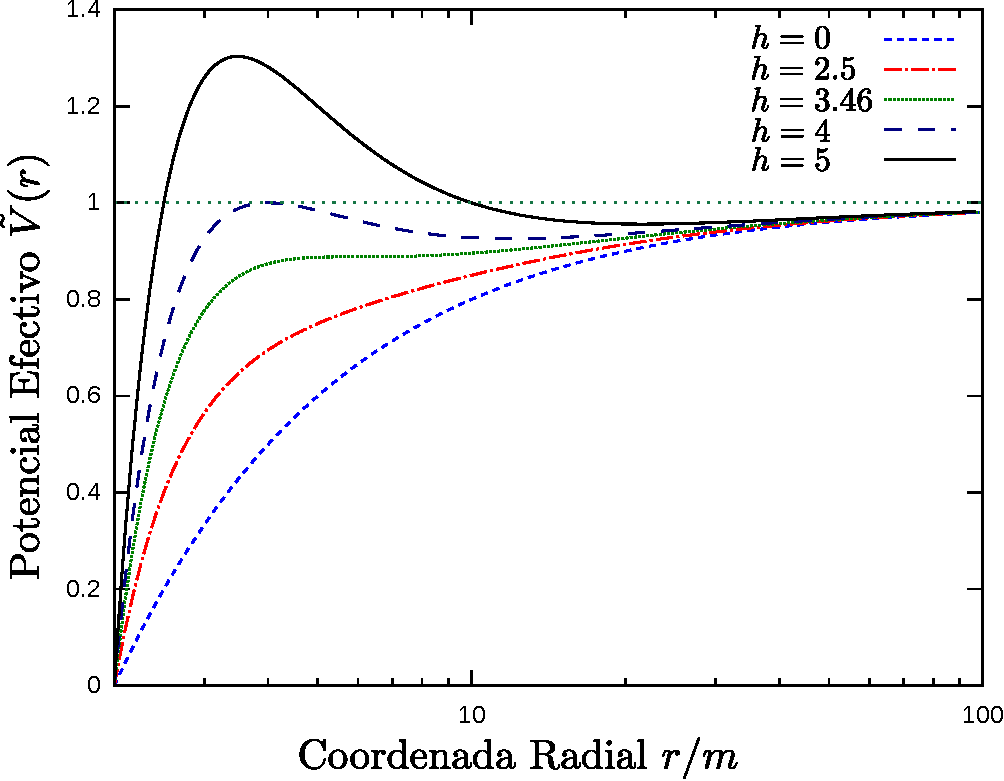
\includegraphics[height=6cm,angle=0]{fig/fig-potencial-efectivo-01.pdf}
\caption{Potencial Efectivo (escala logar'itmica en $r$).} \label{fpe}
\end{center}
\end{figure}

Si $h>2\sqrt{3}$ el potencial tiene entonces un m'aximo en $r=r_A$ y un m'inimo en $r=r_B$. Si $h=2\sqrt{3}$ ambos puntos convergen en un punto de inflexi'on, $r_A=r_B$, y si $h<2\sqrt{3}$ no existen extremos locales.

De acuerdo a lo anterior, existen varios tipos de 'orbitas posibles, dependiendo de los valores de $k$ y $h$:

\begin{itemize}
 \item Si $h<2\sqrt{3}$ y $k<1$ el movimiento radial es acotado, con un m'aximo $r_{\rm max}$ determinado por la igualdad $\tilde{V}(r_{\rm max})=k^2$, pero no existe un m'inimo, de modo que en estos casos la part'icula finalmente cae hacia el cuerpo central.
\item Si $h<2\sqrt{3}$ y $k>1$ la trayectoria no est'a acotada en $r$, correspondiendo a una part'icula que viene desde el infinito y cae hacia el cuerpo central, o que escapa desde 'este hasta el infinito.
\item Si $h>2\sqrt{3}$ y $k^2>\tilde{V}(r_A)$ tenemos una situaci'on similar al caso anterior ($h<2\sqrt{3}$ y $k>1$).
\item Si $h>2\sqrt{3}$ y $k^2=\tilde{V}(r_A)$ existen en principio 'orbitas circulares, con $r=r_{\rm c}=\text{cte.}$, tal que $\tilde{V}(r_{\rm c})=k^2$, pero 'estas son \textit{inestables}. Ver \eqref{ddotr}.
\item Si $h>2\sqrt{3}$, $\tilde{V}(r_B)<k^2<\tilde{V}(r_A)$ y $k>1$ existen 'orbitas no ligadas, donde $r$ puede variar desde un valor m'inimo $r_{\rm min}$ (tal que $\tilde{V}(r_{\rm min})=k^2$, $r_{\rm min}>r_A$) hasta el infinito. Ejemplo de este caso son part'iculas que vienen del infinito, son deflectadas por el cuerpo central y escapan nuevamente al infinito. En este caso son tambi'en posibles 'orbitas que caen inevitablemente al cuerpo central.
\item Si $h>2\sqrt{3}$, $\tilde{V}(r_B)<k^2<\tilde{V}(r_A)$ y $k<1$ existen 'orbitas ligadas, cuyas coordenadas radiales var'ian entre $r_{\rm min}$ y $r_{\rm max}$, con $\tilde{V}(r_{\rm min})=\tilde{V}(r_{\rm max})=k^2$.
\item Si $h>2\sqrt{3}$ y $k^2=\tilde{V}(r_B)$ existen 'orbitas circulares estables, con $r=r_{\rm c}=\text{cte.}$, tal que $\tilde{V}(r_{\rm c})=k^2$.
\item Si $h>2\sqrt{3}$ y $k^2<\tilde{V}(r_B)$ tenemos una situaci'on similar al primer caso aqu'i listado ($h<2\sqrt{3}$ y $k<1$).
\end{itemize}

\subsubsection{'Orbitas circulares}
De acuerdo a la clasificaci'on anterior, estudiamos aqu'i el caso en que $h>2\sqrt{3}$ y $k^2=\tilde{V}(r_B)$. Usando (\ref{rAB}b) encontramos (luego de algo de 'algebra) que las constantes de movimiento apropiadas a un movimiento circular estable deben satisfacer la relaci'on siguiente
% \begin{equation}
%  k^2={\frac {2\left(h^2+h\sqrt{h^2-12}-4\right)^2} {h\left(h+\sqrt{h^2-12}\right)^3}}.
% \end{equation}
\begin{equation}
h_{\rm c}=\frac{r_{\rm c}}{\sqrt{m(r_{\rm c}-3m)}}, \qquad  k_{\rm c}=\frac{\left(1-\frac{2m}{r_{\rm c}}\right)}{\sqrt{1-\frac{3m}{r_{\rm c}}}}.
\end{equation}

Usamos (\ref{kh}a)  para expresar $\dot{t}$ en t'erminos de las constantes de movimiento (recuerde que elegimos $\theta=\pi/2$):
% \begin{equation}
%  \dot{t}_{\rm c}=\frac{k}{1-\frac{2m}{r}}=\sqrt{\frac{2h}{h+\sqrt{h^2-12}}}.
% \end{equation}
\begin{equation}
 \dot{t}_{\rm c}=\frac{1}{\sqrt{1-\frac{3m}{r_{\rm c}}}}.
\end{equation}
Similarmente, a partir de (\ref{kh}b) podemos evaluar $\dot\varphi$ en t'erminos de las constantes de movimiento,
% \begin{equation}
%  \dot\varphi_{\rm c}=\frac{hmc}{r_{\rm c}^2}=\frac{4c}{mh}\frac{1}{\left(h+\sqrt{h^2-12}\right)^2}.
% \end{equation}
\begin{equation}
 \dot\varphi_{\rm c}=\frac{c}{r_{\rm c}}\sqrt{\frac{m}{r_{\rm c}-3m}}.
\end{equation}
Ya que tanto $ \dot{t}_{\rm c}$ como $ \dot\varphi_{\rm c}$ son constantes, podemos integrar las ecuaciones de movimiento directamente, obteniendo
\begin{equation}
 x^\mu(\tau)=(c\dot{t}_{\rm c}\tau,r_{\rm c},\frac{\pi}{2}, \dot\varphi_{\rm c}\tau).
\end{equation}
La menor 'orbita circular estable (``innermost stable circular orbit'', ISCO), se obtiene, de acuerdo a (\ref{rAB}b), en el l'imite $h\to 2\sqrt{3}$. En este caso
\begin{equation}
 r_{\rm c}=6\,m,
\end{equation}
y
\begin{equation}
 k_{_{\rm ISCO}}= \frac{2\sqrt{2}}{3}, \qquad \dot{t}_{_{\rm ISCO}}=\sqrt{2}, \qquad \dot\varphi_{_{\rm ISCO}}=\frac{\sqrt{3}}{18}\frac{c}{m}.
\end{equation}
Por lo tanto, a diferencia del caso newtoniano, \textbf{\textit{la teor'ia gravitacional de Einstein predice un l'imite para la existencia de 'orbitas circulares estables}}. En la teor'ia newtoniana, ellas existen para cada valor de $r>0$, en RG s'olo pueden existir para $r_{\rm c}\ge6m$.

\subsubsection{'Orbitas ligadas no-circulares}
Este es el caso en que $h>2\sqrt{3}$, $\tilde{V}(r_B)<k^2<\tilde{V}(r_A)$ y $k<1$. Para analizar la forma de la trayectoria es conveniente considerar c'omo cambia la coordenada radial en t'erminos de la angular, $r=r(\varphi)$. Para esto, realizamos el cambio de variables correspondiente, de modo que
\begin{equation}
r':=\frac{dr}{d\varphi}=\frac{\frac{dr}{d\tau}}{\frac{d\varphi}{d\tau}}=\frac{
\dot{r}}{\dot{\varphi}}.
\end{equation}
Usando ahora (\ref{kh}b) podemos escribir
\begin{equation}
\dot{r} =\frac{hmc}{r^2}r', \qquad \ddot{r}=\frac{h^2m^2c^2}{r^4}\left[-\frac{2}{r}r'^2+r''\right].
\end{equation}
Adicionalmente, la soluci'on de las ecuaciones de movimiento es m'as simple, tal como en el caso newtoniano, definiendo la variable auxiliar
\begin{equation}
 u:=\frac{1}{r},
\end{equation}
de modo que
\begin{equation}
r' =-\frac{1}{u^2} u',  \qquad r''=\frac{2}{u^3}u'^2-\frac{1}{u^2}u''.
\end{equation}
Con estos cambios, la ecuaci'on (\ref{uuc22})  se transforma en
\begin{equation}
h^2m^2u'^2-k^2+(1-2mu)(1+h^2m^2u^2)=0.
\end{equation}
Derivando esta relaci'on y considerando el caso no circular, es decir $u'\neq 0$, obtenemos
\begin{equation}
u''+u=\frac{1}{mh^2}+3m\,u^2 \label{ecuGR}.
\end{equation}
La ecuaci'on newtoniana correspondiente, ver (\ref{EC1}),  es
\begin{equation}
 u''+u=\frac{1}{mh^2},\label{ecrNew}
\end{equation}
con soluci'on
\begin{equation}
 u_0(\varphi)=\frac{1}{mh^2}\left(1+e\cos\varphi\right).
\end{equation}
% Por lo tanto, el valor m'aximo de $u$ es del orden $u_{\rm max}\approx \frac{1}{mh^2}$.
En estas condiciones, el t'ermino ``extra'' en el lado derecho de (\ref{ecuGR}) es mucho m'as peque\~no que el t'ermino ``newtoniano''. En efecto, definiendo la variable adimensional
\begin{equation}
 w:=mh^2\,u.
\end{equation}
Entonces (\ref{ecuGR})  es equivalente a
\begin{equation}
w''+w=1+\epsilon\,w^2 ,\label{ecwGR}
\end{equation}
con
\begin{equation}
 \epsilon:=\frac{3}{h^2}.
\end{equation}
Usando (\ref{kh}b) encontramos que, en el caso de cuerpos orbitando en campos
d'ebiles (como es el caso en nuestro sistema solar),
\begin{equation}
 \epsilon=\frac{3m^2c^2}{r^4\dot\varphi^2}\approx\frac{3m^2c^2}{r^2v_\varphi^2}
 \approx 3\frac{m^2}{r^2}\frac{c^2}{v_\varphi^2}\approx 3\frac{m}{r}\ll 1.
\end{equation}
En particular para Mercurio $\epsilon\approx 10^{-7}$. Por otro lado $w\approx
1$.

Usando el m'etodo perturbativo, postulamos la siguiente expansi'on para la soluci'on de (\ref{ecuGR}):
\begin{equation}
w(\varphi,\epsilon)=w_0(\varphi)+\epsilon\, w_1(\varphi) +\epsilon^2\,w_2(\varphi)+\mathcal{O}(\epsilon^3), \label{expw}
\end{equation}
donde la soluci'on ``no perturbada'' es
\begin{equation}
 w_0(\varphi)=1+e\cos\varphi ,
\end{equation}
y donde $w_1$, $w_2$ se suponen de orden de magnitud 1. Reemplazando la expansi'on (\ref{expw}) en (\ref{ecuGR}) e igualando t'erminos del mismo orden en potencias de $\epsilon$, obtenemos la siguiente ecuaci'on para la primera perturbaci'on:
\begin{eqnarray}
 w_1''+w_1&=&1+2e\cos\varphi+e^2\cos^2\varphi \\
&=& (1+\frac{e^2}{2})+2e\cos\varphi+\frac{e^2}{2}\cos(2\varphi). \label{ecw1}
\end{eqnarray}
Esta es una ecuaci'on tipo oscilador arm'onico forzado, donde el t'ermino forzante es la superposici'on de un t'ermino constante, un \textit{t'ermino resonante}, y un t'ermino peri'odico no resonante. Su soluci'on es del tipo
\begin{equation}
 w_1(\varphi)=A+B\varphi\sen\varphi+C\cos(2\varphi).
\end{equation}
Reemplazando esta soluci'on general en (\ref{ecw1}) podemos determinar las constantes involucradas:
\begin{equation}
 A=1+\frac{e^2}{2}, \qquad B=e, \qquad C=-\frac{e^2}{6}.
\end{equation}
Con esto, la soluci'on de la ecuaci'on (\ref{ecuGR}) a primer orden en $\epsilon$ adopta la forma:
\begin{equation}\label{solucasi}
 u(\varphi)=\frac{1}{mh^2}\left[1+e\cos\varphi+\epsilon\left[\underbrace{
(1+\frac { e^2 } { 2 } )}_\text{pert.
constante}+\underbrace{e\varphi\sen\varphi}_\text{pert. ``secular''}
-\underbrace{\frac{e^2 }{6} \cos(2\varphi)}_\text{pert. peri'odica}\right ]
\right ] +\mathcal{O}(\epsilon^2).
\end{equation}
Usando ahora
\begin{equation}
 \cos(\epsilon\varphi) =1+\mathcal{O}(\epsilon^2), \qquad
\sen(\epsilon\varphi) =\epsilon\varphi+\mathcal{O}(\epsilon^3),
\end{equation}
podemos escribir los t'erminos newtonianos y de perturbaci'on secular como
\begin{equation}
 \cos\varphi+\epsilon\varphi\sen\varphi=\cos\left[(1-\epsilon)\varphi\right]
+\mathcal{O}(\epsilon^2).
\end{equation}
An'alogamente, para la perturbaci'on peri'odica podemos usar
\begin{equation}
 \epsilon\cos(2\varphi)=\epsilon\cos\left[2(1-\epsilon)\varphi\right]+\mathcal{O}(\epsilon^2).
\end{equation}
Con esto podemos expresar nuestra soluci'on como
\begin{equation}\marginnote{Trayectoria perturbada}
 \boxed{u(\varphi)=\frac{1}{mh^2}\left[1+\epsilon(1+\frac { e^2 } { 2 }
)+e\cos\left[(1-\epsilon)\varphi\right] -\frac { e^2
}{6}\epsilon\cos[2(1-\epsilon)\varphi]\right ] +\mathcal{O}(\epsilon^2).} \label{solu1}
\end{equation}
Esta forma de la soluci'on a primer orden tiene la ventaja que revela m'as claramente que la 'orbita (nuevamente, a primer orden en $\epsilon$) \textit{es peri'odica en $\varphi$, pero con un periodo angular distinto de $2\pi$}. Como consecuencia, la 'orbita no se cierra luego de una revoluci'on completa. Este hecho implica en particular un \textit{corrimiento del perihelio de la 'orbita}.

\subsubsection{El Avance del Perihelio de Mercurio}

De (\ref{solu1}) vemos que, a primer orden en $\epsilon$, el periodo angular de la 'orbita no es $2\pi$, sino $2\pi/(1-\epsilon)>2\pi$. Esto significa que la 'orbita retornar'a a una misma distancia dada del centro de fuerzas (por ejemplo, el perihelio) s'olo luego de realizar algo m'as que una rotaci'on completa en torno al centro de fuerzas, en un 'angulo de $2\pi/(1-\epsilon)$. En otras palabras, el \textit{corrimiento angular} de la 'orbita es dado por
\begin{figure}[H]
 \begin{center}
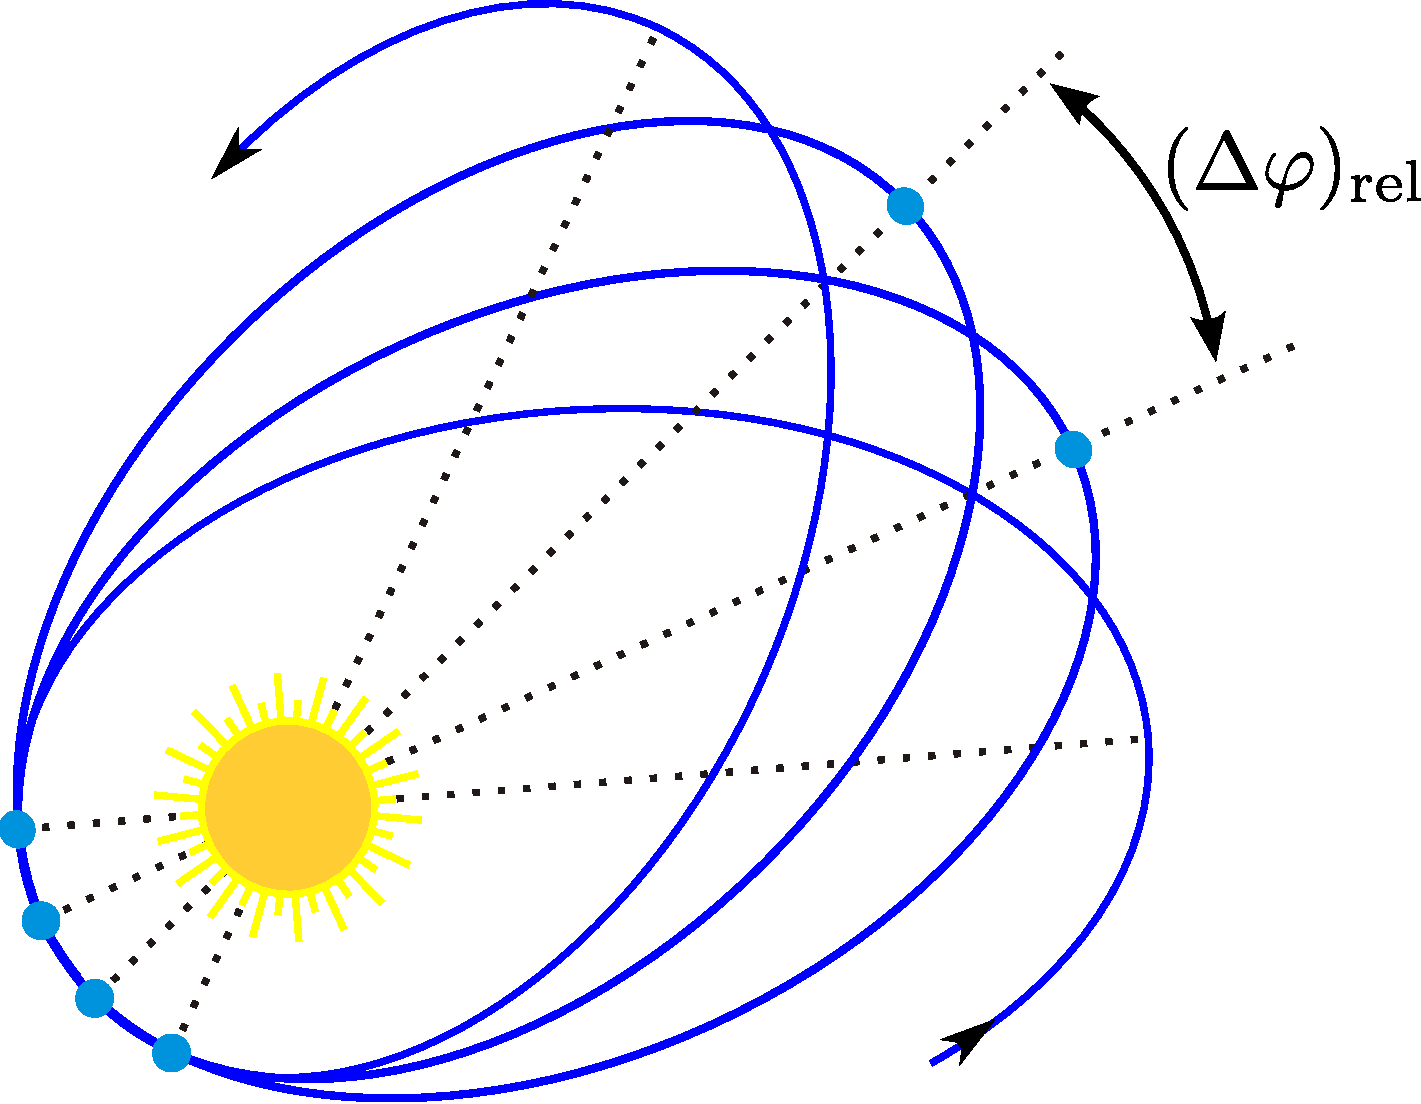
\includegraphics[height=5cm]{fig/fig-precesion-02.pdf}
\caption{Corrimiento del perihelio (adaptada a partir de \href{http://en.wikipedia.org/wiki/File:Perihelion_precession.svg}{esta} figura original).}
\end{center}
\end{figure}
\begin{equation}
\Delta\varphi=\frac{2\pi}{1-\epsilon}-2\pi=2\pi\epsilon+\mathcal{O}(\epsilon^2)=\frac{6\pi}{h^2}+\mathcal{O}(\epsilon^2).
\end{equation}
Podemos expresar $\epsilon$ en t'erminos del semieje mayor y la excentricidad de la 'orbita, ya que
\begin{equation}
a:=\frac{r_{\rm min}+r_{\rm max}}{2}=\frac{mh^2}{1-e^2}+\mathcal{O}(\epsilon).
\end{equation}
As'i obtenemos, a primer orden,
\begin{equation}
 (\Delta\varphi)_{\rm rel}\approx\frac{6\pi m}{a(1-e^2)},
\end{equation}
o, en t'erminos de la masa del cuerpo central:
\begin{equation}\marginnote{Avance periastro}
 \boxed{(\Delta\varphi)_{\rm rel}\approx \frac{6\pi GM}{ac^2(1-e^2)}.}
\end{equation}

Esta expresi'on fue derivada por Einstein en 1915 y aplicada al caso de la 'orbita de Mercurio \cite{Einstein15}. El avance del perihelio de Mercurio era un fen\'omeno conocido antes de la formulaci'on de la teor\'ia de la Relatividad General, ya que Le Verrier \cite{LeVerrier} public'o en 1859 sus observaciones y c'alculos en los que dejaba en evidencia un \textit{avance an'omalo} de $\approx 45\pm 5$''/siglo  (valor citado por Einstein en \cite{Einstein15}). Este valor an'omalo es el resultante de restar el valor esperado de acuerdo a la teor'ia de newton al valor observado\footnote{Luego de tambi'en sustraer el efecto de la \href{http://en.wikipedia.org/wiki/Axial_precession}{precesi\'on general}. Ver referencia \cite{Clemence47} para m'as detalles.} (de la 'epoca) de $\approx 574$''/siglo.  De acuerdo a Clemence (1947) \cite{Clemence47} las mayores contribuciones newtonianas al corrimiento del perihelio de Mercurio son: Venus ($\approx 278$''/siglo), J'upiter ($\approx 153$''/siglo), la Tierra ($\approx 90$''/siglo), Saturno ($\approx 7$''/siglo), Marte ($\approx 2.5$''/siglo), Urano ($\approx 0.14$''/siglo), Neptuno ($\approx 0.042$''/siglo). Con esto, el corrimiento an'omalo asciende a $\approx 43$''/siglo, valor no pod'ia ser calculado usando la teor'ia newtoniana, y que fue entonces explicado por la nueva teor'ia de Einstein.

Para el caso de Mercurio\footnote{Ver, por ejemplo, \url{http://nssdc.gsfc.nasa.gov/planetary/factsheet/mercuryfact.html}.}  $a\approx 57.91\times 10^6\text{\,km}$, $e\approx 0.2056$. Adem'as, $GM_\odot/c^2\approx 1.48\text{\,km}$. Con esto, la predicci'on relativista para el corrimiento del perihelio de Mercurio asciende a $(\Delta\varphi)_{\rm rel}\approx 5.03\times 10^{-7}{\,\rm rad/rev}\approx 0.104$''/rev. Como el periodo orbital de Mercurio es $T\approx 87.97\text{ d'ias}\approx 2,41\times 10^{-3}\text{ siglo}$, entonces  $(\Delta\varphi)_{\rm rel}\approx 43$''/siglo. El valor aceptado actualmente para la predicci'on relativista es de $(\Delta\varphi)_{\rm rel}\approx 42.98$''/siglo, ver \cite{NW86}. Este resultado est'a en completo acuerdo con el resultado observacional aceptado actualmente, de $42.98(1.000\pm 0.001)$''/siglo. Ver \cite{Will06}, secci'on 3.5, para detalles adicionales.

La predicci'on de RG para el corrimiento del perihelio ha sido adem'as verificada en nuestro sistema solar para las 'orbitas de Venus, la Tierra y Marte. En esos casos el corrimiento relativista asciende a aproximadamente $8.65$''/siglo, $3.85$''/siglo y $1.36$''/siglo, respectivamente \cite{OR94}. Una de las mejores verificaciones actualmente disponible es la correspondiente al corrimiento del perihelio de la 'orbita del pulsar binario de Hulse \& Taylor PRS 1913+16, para el cual el corrimiento es de aproximadamente 13''/rev (y el periodo de rotaci'on es algo menor que 8 horas!) \cite{Taylor93}.

\subsection{Desv'io de la luz}

En este caso, realizaremos un c'alculo similar al correspondiente a trayectorias tipo tiempo, con la diferencia que la ecuaci'on de la geod'esica, usando un par'ametro arbitrario $\lambda$, adopta la forma
\begin{equation}
\frac{d^2x^\mu}{d\lambda^2}+\Gamma^\mu_{\nu\rho}\frac{dx^\nu}{d\lambda}\frac{dx^\rho}{d\lambda}=f(\lambda)\frac{dx^\mu}{d\lambda},
\end{equation}
De este modo las ecuaciones de movimiento toman la forma (aqu'i denotamos $\dot{(\ \,)}:={d(\ \,)}/{d\lambda}$):
\begin{eqnarray}
\frac{1}{\left(1-\frac{2m}{r}\right)}\frac{d\ }{d\lambda}\left[\left(1-\frac{2m}{r}\right)\dot{t}\right]&=&f\,\dot{t}, \label{egSl0}\\
\ddot{r}+\frac{mc^2(r-2m)}{r^3}\,\dot{t}^2-\frac{m}{r\left(
r-2m\right) }\,\dot{r}^2-(r-2m) \left[ \dot{\theta}^2+\sen
^2\theta \dot{\varphi}^2\right] &=&f\,\dot{r}, \label{egSl1}\\
\ddot{\theta}+\frac{2}{r}\dot{r}\dot{\theta}-\sen \theta \cos \theta
\dot{\varphi}^2 &=&f\,\dot{\theta}, \label{egSl2}\\
\frac{1}{r^2\sen^2\theta}\frac{d\ }{d\lambda}\left[r^2\sen^2\theta\dot{\varphi}\right] &=&f\,\dot{\varphi}.\label{egSl3}
\end{eqnarray}%
Note que hemos factorizado los t'erminos al lado izquierdo de (\ref{egSl0}) y (\ref{egSl3}). Nuevamente, el movimiento est'a confinado a un plano, que podemos elegir como el plano ecuatorial, es decir, con $\theta(\lambda)=\pi/2$. Verificamos que esta soluci'on para $\theta$ satisface (\ref{egSl2}). Tal como en el caso tipo tiempo, finalmente nos concentraremos en la forma de la trayectoria. Por esto, elegiremos como par'ametro al 'angulo $\varphi$, es decir, $\lambda:=\varphi$. Con esto, $\dot{\varphi}=1$ y podemos determinar la funci'on $f$ correspondiente a partir de (\ref{egSl3}):
\begin{equation}
f=\frac{d\ }{d\varphi}\ln\left[r^2\right]=\frac{2}{r}r'.
\end{equation}
Introduciendo esta funci'on en (\ref{egSl0}) obtenemos, luego de una simple 'algebra,
\begin{equation}
\frac{d\ }{d\varphi}\ln\left[\frac{r^2}{\left(1-\frac{2m}{r}\right)t'}\right]=0,
\end{equation}
que expresa el hecho que existe una cantidad conservada en el movimiento:
\begin{equation}\label{ccl}
 \frac{r^2}{\left(1-\frac{2m}{r}\right)}\frac{d\varphi}{dt}=:\frac{c}{\alpha}.
\end{equation}
Aqu'i, para conveniencia posterior, hemos introducido $\alpha$ como constante, con dimensiones $[\alpha]=L^{-1}$, determinada por las condiciones iniciales del movimiento.

Por otro lado, la ecuaci'on radial (\ref{egSl1}) se reduce a
\begin{equation}
 r''+\frac{mc^2(r-2m)}{r^3}\,t'^2-\frac{m}{r\left(r-2m\right) }\,r'^2-(r-2m) =\frac{2}{r}r'^2. \label{ecr2l}
\end{equation}

Tal como en el caso tipo tiempo, esta ecuaci'on puede derivarse de la ecuaci'on de primer orden, en este caso, de la condici'on $g_{\mu\nu}\dot{x}^\mu\dot{x}^\nu=0$. Esta condici'on implica que
\begin{equation}
\left(1-\frac{2m}{r}\right)c^2\left(\frac{dt}{d\varphi}\right)^2-\frac{1}{\left(1-\frac{2m}{r}\right)}\left(\frac{dr}{d\varphi}\right)^2-r^2=0. \label{e2orl}
\end{equation}
Usando (\ref{ccl}) para expresar $dr/d\varphi$ en t'erminos de $r$ y la constante de moviento $\alpha$, la condici'on (\ref{e2orl}) se reduce a
\begin{equation}\label{ecrpf}
 r'^2+r^2-2mr-\alpha^2r^4=0,
\end{equation}
donde $'$ denota la derivada con respecto a $\varphi$.

Introduciendo ahora $u:=1/r$ transformamos esta ecuaci'on en
\begin{equation}
 u'^2+u^2=\alpha^2+2mu^3. \label{ecul0}
\end{equation}
Derivando esta ecuaci'on llegamos a una ecuaci'on de segundo orden en las derivadas de $u$ que, tal como en el caso tipo tiempo, es equivalente a la ecuaci'on (\ref{ecr2l}):
\begin{equation}
 u''+u=3mu^2. \label{ecglrg}
\end{equation}
Esta ecuaci'on es la an'aloga a (\ref{ecuGR}). Tal como en el caso anterior, el t'ermino introducido por la teor'ia de RG es $3mu^2$. Puede comprobarse que la ecuaci'on newtoniana, que corresponde al l'imite $m\to 0$, es
\begin{equation}
 u''+u=0, \label{ecglnew}
\end{equation}
y que \textit{sus soluciones son l'ineas rectas}. En efecto, una soluci'on general de (\ref{ecuGR}) puede expresarse en la forma siguiente:
\begin{equation}
 u_0(\varphi)=\frac{1}{D}\sen(\varphi-\varphi_0),
\end{equation}
donde $D$ es una constante con dimensiones de longitud y $\varphi_0$ una constante angular. Entonces tendremos que
\begin{equation}
x=r\cos\varphi=D\frac{\cos\varphi}{\sen(\varphi-\varphi_0)}, \qquad
y=r\sen\varphi=D\frac{\sen\varphi}{\sen(\varphi-\varphi_0)}.
\end{equation}
Una simple 'algebra permite entonces relacionar $x$ con $y$, obteniendo
\begin{equation}
 y=\frac{D}{\cos\varphi_0}+\left(\tan\varphi_0\right)x. \label{recta}
\end{equation}
La expresi'on (\ref{recta}) describe una recta en el plano $x-y$, siendo $D$ la \textit{distancia m'inima de la recta al origen} y $\varphi_0$ el 'angulo que forma la recta con el eje $x$. Ver figura \ref{fig:recta}.
\begin{figure}[H]
 \begin{center}
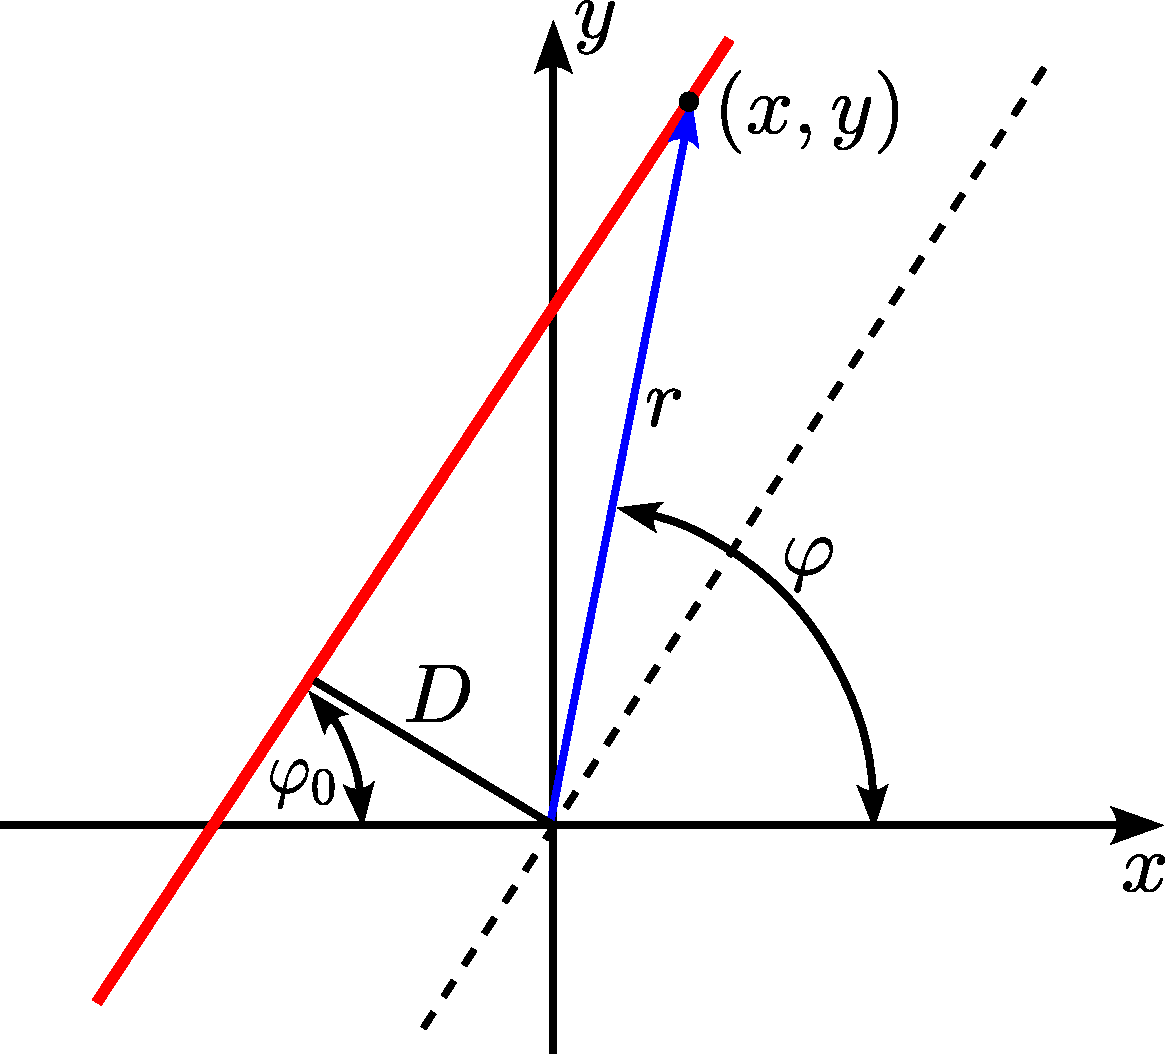
\includegraphics[height=6cm]{fig/fig-recta.pdf}
\caption{Soluci'on newtoniana para el movimiento del rayo de luz.}
\label{fig:recta}
\end{center}
\end{figure}

Determinaremos nuevamente una soluci'on aproximada de (\ref{ecglrg}). Primero definimos la variable adimensional $w(\varphi):=Du(\varphi)$. Con esto (\ref{ecglrg}) se transforma en
\begin{equation}
 w''+w=\epsilon\, w^2, \label{ecglrgw}
\end{equation}
que tiene como soluci'on ``sin perturbar'' a
\begin{equation}
 w_0(\varphi)=\sen(\varphi-\varphi_0). \label{w0l}
\end{equation}
La constante $\epsilon$ tiene el valor
\begin{equation}
 \epsilon:=\frac{3m}{D},
\end{equation}
que es mucho menor que 1, ya que suponemos que el rayo de luz pasa suficientemente lejos del centro de fuerzas de modo que $D\gg m$. Suponemos adem'as que $w\approx 1$. Con estos ingredientes determinaremos una soluci'on perturbativa de la forma (\ref{expw}), con $w_0$ dado por (\ref{w0l}). Introduciendo la expansi'on (\ref{expw}) y usando (\ref{w0l}) encontramos la ecuaci'on para la primera perturbaci'on $w_1$:
\begin{equation}
 w_1''+w_1=\sen^2(\varphi-\varphi_0). \label{ecw1l}
\end{equation}
La soluci'on general de esta ecuaci'on es de la forma
\begin{equation}
 w_1(\varphi)=A+B\cos(\varphi-\varphi_0+\beta)+C\cos^2(\varphi-\varphi_0).
\end{equation}
Substituyendo esta expresi'on en (\ref{ecw1l}) encontramos que $A=C=1/3$, mientras que las constantes $B$ y $\beta$ pueden adoptar valores arbitrarios. Sin embargo, sin p'erdida de generalidad es posible elegir\footnote{En efecto, si $B\neq 0$ y $\beta\neq 0$, la soluci'on puede reescribirse, \textit{a primer orden en} $\epsilon$ como
\begin{equation*}
u(\varphi)=\frac{1}{\tilde{D}}\left[\sen(\varphi-\tilde{\varphi}_0)+\frac{m}{\tilde{D}}\left(1+\cos^2(\varphi-\tilde{\varphi_0})\right)\right]+\mathcal{O}(\epsilon^2),
\end{equation*}
con $\tilde{D}:=D/(1-\epsilon B\sen\beta)$ y $\tilde{\varphi}_0:=\varphi_0-\epsilon B\cos\beta$. Esta expresi'on es equivalente a (\ref{solw1l}).} $B=\beta=0$. As'i, nuestra soluci'on a primer orden adopta la forma siguiente:
\begin{equation}\marginnote{Soluci'on pertubada rayo de luz}
 \boxed{u(\varphi)=\frac{1}{D}\left[\sen(\varphi-\varphi_0)+\frac{m}{D}\left[1+\cos^2(\varphi-\varphi_0)\right]\right]+\mathcal{O}(\epsilon^2).} \label{solw1l}
\end{equation}
Para calcular el \textit{'angulo de desv'io} de la luz, $\delta$, necesitamos los 'angulos $\delta_1$ y $\delta_2$ en que la trayectoria se desv'ia de la recta no perturbada, para $t\to -\infty$ y $t\to +\infty$, respectivamene. Estos 'angulos corresponden a un 'angulo inicial $\varphi_{\rm i}=\varphi_0+\pi+\delta_1$ y final $\varphi_{\rm f}=\varphi_0-\delta_2$, y pueden ser determinados por la condici'on que en cada caso $r\to\infty$ o, equivalentemente $u=0$. El 'angulo total de desv'io es entonces $\delta=\delta_1+\delta_2$. Reemplazamos por tanto $\varphi=\varphi_{\rm i}=\varphi_0+\pi+\delta_1$ en la condici'on $u(\varphi_{\rm i})$ obtenemos, a primer orden en $\delta_1$:
\begin{eqnarray}
 0&=&u(\varphi_{\rm i})\\
&=&\frac{1}{D}\left[\sen(\pi+\delta_1)+\frac{m}{D}\left(1+\cos^2(\pi+\delta_1)\right)\right] \\
&=&\frac{1}{D}\left[-\sen\delta_1+\frac{m}{D}\left(1+\cos^2\delta_1)\right)\right] \\
&=&\frac{1}{D}\left[-\delta_1+\frac{m}{D}\left(1+1\right)\right]+\mathcal{O}(\delta_1^2).
\end{eqnarray}
Por lo tanto, obtenemos,
\begin{equation}
 \delta_1=\frac{2m}{D}.
\end{equation}
Similarmente, para $\varphi_{\rm f}=\varphi_0-\delta_2$ encontramos:
\begin{eqnarray}
 0&=&u(\varphi_{\rm f})\\
&=&\frac{1}{D}\left[-\sen\delta_2+\frac{m}{D}\left(1+\cos^2\delta_2\right)\right] \\
&=&\frac{1}{D}\left[-\delta_2+\frac{m}{D}\left(1+1\right)\right]+\mathcal{O}(\delta_2^2),
\end{eqnarray}
de modo que
\begin{equation}
 \delta_2=\frac{2m}{D}.
\end{equation}
As'i obtenemos que el 'angulo total de desv'io es
\begin{equation}
 \delta\approx\frac{4m}{D},
\end{equation}
o, en t'erminos de la masa del cuerpo central\footnote{Note que, en estricto rigor, la constante $D$ no es exactamente el valor m'inimo de la coordenada radial en la trayectoria del fot'on. La soluci'on (\ref{solw1l}) implica que el m'inimo de $r$ (m'aximo de $u$) se obtiene para $\varphi=\varphi_0+\pi/2$, y que a primer orden $r_{\rm min}=D/(1+m/D)\approx D-m$. La diferencia entre $D$ y $r_{\rm min}$ es por esto muy peque\~na y despreciable en el contexto de de la aproximaci'on usada.\label{fn8}},
\begin{equation}\marginnote{'Angulo de desv'io} \label{dlRG}
 \boxed{\delta\approx\frac{4GM}{c^2D}.}
\end{equation}

En 1911 Einstein presenta un primer c'alculo para el 'angulo de desv'io de la luz en un campo gravitacional, basado en el principio de equivalencia, pero a'un en el contexto de la teor'ia newtoniana. El valor calculado de esta forma resulta ser \textit{la mitad} del 'angulo \eqref{dlRG} que predice teor'ia de Relatividad General completa. Ver \cite{Einstein11}, p'agina 908. Es interesante notar adem'as que si se considera la teor'ia newtoniana de la gravitaci'on y a los fotones como part'iculas (masivas) que son atraidas por el Sol y que se mueven con rapidez $c$, tambi'en se obtiene el resultado correspondiente a la mitad de \eqref{dlRG}. Ver \cite{Will88} para mayores detalles.  Por otro lado, el resultado \eqref{dlRG} fue presentado por Einstein por primera vez en su paper de 1916 \cite{Einstein16} (ecuaci'on 74, p'agina 822).

Note tambi'en que, de acuerdo a \eqref{dlRG}, la teor'ia de RG predice un 'angulo de desv'io \textit{independiente de la frecuencia de la radiaci'on}.

En el caso de rayos de luz pasando muy cerca de la superficie del Sol\footnote{Ver, por ejemplo, \url{http://nssdc.gsfc.nasa.gov/planetary/factsheet/sunfact.html}.}, $D\approx R_\odot\approx 6.96\times 10^5\text{\,km}$, y entonces
\begin{equation}
\delta_\odot\approx\frac{4GM}{c^2R_\odot}\approx 4\left(\frac{1.48\text{\,km}}{6.96\times 10^5\text{\,km}}\right)\approx 4\times 2.13\times 10^{-6}{\rm\, rad}\approx 8.52\times 10^{-6}{\rm\, rad}\approx 1.75\text{''}.
\end{equation}

La observaci'on de este efecto constituy'o la \textit{primera verificaci'on experimental de una predicci'on} de la teor'ia de gravitaci'on de Einstein. El desv'io de la luz fue medido en Mayo de 1919 por Eddington\footnote{Sir Arthur Eddington (1882-1944) astrof'isico brit'anico. Ver, por ejemplo, \url{http://es.wikipedia.org/wiki/Arthur_Stanley_Eddington}.} y colaboradores, a partir de mediciones 'opticas de las posiciones de estrellas cercanas al Sol, medidas durante un eclipse total de Sol, observado desde las islas atl'anticas de Sobral y Principe \cite{DED19}. Estos experimentos obtuvieron un resultado consistente con la predicci'on relativista, pero s'olo con un 30\% de precisi'on. Sin embargo, los resultados s'i permit'ian excluir un resultado nulo o la predicci'on ``cuasi-newtoniana'' (la mitad del valor de RG, es decir, $\approx 0.87$''). Se efectuaron nuevas medidas durante eclipses posteriores. En el del 30 de Junio de 1973 los resultados concordaban con la predicci'on de RG con un error del 10\%. Uno de las mayores fuentes de error en este tipo de observaci'on es causada por la corona solar, que tambi'en curva los rayos que pasan por ella. Actualmente, la precisi'on alcanzada por los sistemas VLBI (Very Large Baseline Interferometry) han permitido mejorar sustancialmente la confirmaci'on observacional de la predicci'on de RG para el desv'io de la luz, con una desviaci'on de 0.1\% \cite{SDLG04,Will06}.

\subsection{Redshift Gravitacional}\label{sec:redshift}
Revisaremos aqu'i la predicci'on para el redshift gravitacional (dilataci'on temporal gravitacional). En particular, derivaremos la expresi'on exacta para el redshift medido por dos observadores ``en reposo'' en el espaciotiempo de Schwarzschild. En particular consideraremos fotones que ``escapan'' del centro de fuerzas de manera radial. En este caso, debido a la simetr'ia esf'erica podemos considerar que los fotones se mueven en trayectorias con $\theta=\pi/2$ y $\varphi=0$.

De la condici'on de curva nula para el fot'on $g_{\mu\nu}dx^\mu dx^\nu=0$ obtenemos
\begin{equation}
 \left(1-\frac{2m}{r}\right)c^2dt^2-\frac{dr^2}{ \left(1-\frac{2m}{r}\right)}=0.
\end{equation}
Por lo tanto,
\begin{equation}
 c\,dt=\pm\frac{dr}{ \left(1-\frac{2m}{r}\right)}.
\end{equation}
Los signos positivo y negativo corresponden a fotones ``escapando desde'' y ``cayendo hacia'' el centro de fuerzas, respectivamente. Para el primer caso, tenemos entonces que
\begin{eqnarray}
 c(t-t_0)&=&\int^r_{r_0}\frac{dr}{\left(1-\frac{2m}{r}\right)} \\
&=&\left.\left(r+2m\ln|r-2m|\right)\right|^r_{r_0} \\
&=&r-r_0+2m\ln\left(\frac{r-2m}{r_0-2m}\right).
\end{eqnarray}
En otras palabras,
\begin{equation} \label{tferf}
 t=t_0+\frac{1}{c}\left[r-r_0+2m\ln\left(\frac{r-2m}{r_0-2m}\right)\right].
\end{equation}
Esta relaci'on define en forma impl'icita la ecuaci'on de la trayectoria, exacta en el espaciotiempo de Schwarzschild, $r(t)$, del fot'on escapando radialmente. Podemos verificar  aqu'i lo usado en la discusi'on del redshift gravitacional en la secci'on (\ref{zg1}): que $(\Delta t)_{\rm e}=(\Delta t)_{\rm r}$. En efecto, si un fot'on es emitido en el evento con coordenadas $x^\mu_{{\rm e},1}=(t_0,r_0,\pi/2,0)$ entonces 'este llega a un punto con coordenada radial $r$ en el evento $x^\mu_{{\rm r},1}=(t,r,\pi/2,0)$, donde $t$ es dado por (\ref{tferf}). Como (\ref{tferf}) es lineal en $t_0$ tendremos que si otro fot'on es enviado desde $r_0$ en el evento $x^\mu_{{\rm e},2}=(t_0+(\Delta t)_{\rm e},r_0,\pi/2,0)$, entonces llegar'a a $r$ en el evento $x^\mu_{{\rm e},2}=(t+(\Delta t)_{\rm e},r,\pi/2,0)$. En otras palabras, $(\Delta t)_{\rm e}=(\Delta t)_{\rm r}$. Este es un resultado general, v'alido para todo espaciotiempo estacionario (es decir, en que la m'etrica es independiente de la coordenada temporal).

Por otro lado, los tiempos propios asociados a observadores ``en reposo'' en el punto de emisi'on y recepci'on, es decir, cuyas l'ineas de mundo tienen coordenada radial constate $r_{\rm e}$ y $r_{\rm r}$ respectivamente, quedan determinados por
\begin{equation}
 ds^2=c^2d\tau^2=\left(1-\frac{2m}{r}\right)c^2dt^2,
\end{equation}
de modo que
\begin{equation}
\Delta\tau_{\rm e}=\sqrt{1-\frac{2m}{r_{\rm e}}}\, (\Delta t)_{\rm e}, \qquad
\Delta\tau_{\rm r}=\sqrt{1-\frac{2m}{r_{\rm r}}}\, (\Delta t)_{\rm r}.
\end{equation}
Con estos ingredientes, obtenemos
\begin{equation}\marginnote{Dilataci'on temporal gravitacional}\label{rgsch}
\boxed{\frac{\Delta\tau_{\rm r}}{\Delta\tau_{\rm e}}=\sqrt{\frac{1-\frac{2m}{r_{\rm r}}}{1-\frac{2m}{r_{\rm e}}}}}.
\end{equation}
Compare esta expresi'on con aquella encontrada en el l'imite de campo d'ebil, expresiones  (\ref{zapp1}) y (\ref{zapp2}).

\subsection{Tiempo de Vuelo (Efecto Shapiro)*}
Aqu'i estudiaremos la predicci'on de la teor'ia de Einstein de la gravitaci'on en lo que respecta al \textit{tiempo de vuelo} de se\~nales luminosas en la m'etrica de Schwarzschild.

Para obtener informaci'on del tiempo de vuelo de una se\~nal luminosa debemos analizar c'omo cambia la coordenada temporal $t$ a lo largo de la l'inea de mundo del rayo de luz.
Usando (\ref{ccl}) podemos escribir
\begin{equation}
\frac{dr}{dt}=\frac{dr}{d\varphi}\frac{d\varphi}{dt}=r'\frac{mc}{\alpha}\left(1-\frac{2m}{r}\right)\frac{1}{r^2}.
\end{equation}
Reemplazando ahora la expresi'on para $r'$ determinada por la relaci'on (\ref{ecrpf}) encontramos que
\begin{equation}
\frac{1}{c}\frac{dr}{dt}=\pm\, I(r),
\end{equation}
donde hemos definido
\begin{equation}
I(r):=\frac{1}{\alpha}\left(1-\frac{2m}{r}\right)\sqrt{\alpha^2+\frac{2m}{r^3}-\frac{1}{r^2}}.
\end{equation}
Ahora aplicamos esta expresi'on al caso en que el fot'on se mueve desde un punto con coordenadas $(ct_T,r_T,\pi/2,\varphi_T)$ hacia el centro de fuerzas, hasta el punto $(ct_0,r_0,\pi/2,\varphi_0)$ de m'aximo acercamiento. En este primer tramo $dr/dt<0$ y entonces
\begin{equation}\label{Dti1}
c\,(t_0-t_T)=-\int^{r_0}_{r_T}\frac{dr}{I(r)}.
\end{equation}
En el segundo tramo, desde $(ct_0,r_0,\pi/2,\varphi_0)$ hasta $(ct_V,r_V,\pi/2,\varphi_V)$, tenemos que $dr/dt>0$ y entonces
\begin{equation}\label{Dti2}
c\,(t_V-t_0)=\int_{r_0}^{r_V}\frac{dr}{I(r)}.
\end{equation}
El intervalo total de coordenada temporal en el proceso de vuelo (``de ida'') es entonces dado por $t_V-t_T$. Usando (\ref{Dti1}) y (\ref{Dti2}) obtenemos
\begin{eqnarray}
c\,(t_V-t_T)&=&\int_{r_0}^{r_V}\frac{dr}{I(r)}-\int^{r_0}_{r_T}\frac{dr}{I(r)} \\
&=&\int_{r_0}^{r_V}\frac{dr}{I(r)}+\int_{r_0}^{r_T}\frac{dr}{I(r)}. \label{cDtI}
\end{eqnarray}
Para evaluar esta expresi'on es necesario escribir $\alpha$ en t'erminos de $r_0=r_{\rm min}$, la coordenada radial m'inima al centro de fuerzas sobre la trayectoria del fot'on. Esta coordenada m'inima se encuentra, ver nota al pie \ref{fn8}, para el 'angulo $\varphi_{\rm min}=\varphi_0+\pi/2$ y satisface $u(\varphi_{\rm min})=1/r_{\rm min}$, $u'(\varphi_{\rm min})=0$, con
\begin{equation}
 r_0=D\left(1-\frac{m}{D}\right)+\mathcal{O}(\epsilon^2).
\end{equation}
Usando estas condiciones, la relaci'on (\ref{ecul0}) implica que
\begin{equation}
 \alpha^2=\frac{1}{r^2_0}\left(1-\frac{2m}{r_0}\right),
\end{equation}
y entonces
\begin{equation}
\alpha=\frac{1}{r_0}\left(1-\frac{m}{r_0}\right)+\mathcal{O}(\epsilon^2).
\end{equation}
Con esto, podemos expresar la funci'on $I(r)$ como
\begin{eqnarray}
 I(r)&=&\frac{1}{\alpha}\left(1-\frac{2m}{r}\right)\sqrt{\alpha^2+\frac{2m}{r^3}-\frac{1}{r^2}} \\
&=&\left(1-\frac{2m}{r}\right)\left(1+\frac{m}{r_0}\right)\sqrt{1-\frac{2m}{r_0}-\frac{2mr_0^2}{r^3}-\frac{r_0^2}{r^2}} +\mathcal{O}(\epsilon^2)\\
&=&\left(1-\frac{2m}{r}+\frac{m}{r_0}\right)\sqrt{1-\frac{r_0^2}{r^2}-\frac{2m}{r_0}\left(1-\frac{r_0^3}{r^3}\right)}+\mathcal{O}(\epsilon^2) \\
&=&\left(1-\frac{2m}{r}+\frac{m}{r_0}\right)\left[\sqrt{1-\frac{r_0^2}{r^2}}+\frac{1}{2\sqrt{1-\frac{r_0^2}{r^2}}}\left(-\frac{2m}{r_0}\right)\left(1-\frac{r_0^3}{r^3}\right)\right] +\mathcal{O}(\epsilon^2)\\
&=&\left(1-\frac{2m}{r}+\frac{m}{r_0}\right)\sqrt{1-\frac{r_0^2}{r^2}}\left[1-\frac{m}{r_0}\frac{\left(1-\frac{r_0^3}{r^3}\right)}{1-\frac{r_0^2}{r^2}}\right] +\mathcal{O}(\epsilon^2)\\
&=&\left(1-\frac{2m}{r}+\frac{m}{r_0}\right)\sqrt{1-\frac{r_0^2}{r^2}}\left[1-\frac{m}{r_0}\frac{\left(1+\frac{r_0}{r}+\frac{r_0^2}{r^2}\right)}{1+\frac{r_0}{r}}\right]+\mathcal{O}(\epsilon^2) \\
&=&\sqrt{1-\frac{r_0^2}{r^2}}\left[1-\frac{mr_0}{r(r+r_0)}-\frac{r_0}{r}\right]+\mathcal{O}(\epsilon^2).
\end{eqnarray}
De esta forma, obtenemos
\begin{equation}
 \frac{1}{I(r)}=\frac{1}{\sqrt{1-\frac{r_0^2}{r^2}}}\left[1+\frac{mr_0}{r(r+r_0)}+\frac{r_0}{r}\right]+\mathcal{O}(\epsilon^2),
\end{equation}
y entonces
\begin{equation}
 \int\frac{dr}{I(r)}=\sqrt{r^2-r_0^2}+2m\ln\left(r+\sqrt{r^2-r_0^2}\right)+m\sqrt{\frac{r-r_0}{r+r_0}}+\mathcal{O}(\epsilon^2).
\end{equation}
Con este resultado podemos evaluar el intervalor $(\Delta t)_{\rm ir}$ de ``ida y regreso''\footnote{Note que este intervalo es en rigor el intervalo de coordenada temporal. El tiempo propio que un observador en $r_T$ registra en el viaje de ida y regreso del fot'on es dado, a primer orden, por $(\Delta\tau)_{\rm ir}=(1-m/r_T)(\Delta t)_{\rm ir}$.} que, de acuerdo a (\ref{cDtI}), es entonces dado por
\begin{eqnarray}
\frac{c}{2}\,(\Delta t)_{\rm ir}&=&\sqrt{r_V^2-r_0^2}+\sqrt{r_T^2-r_0^2}+2m\ln\left[\frac{\left(r_V+\sqrt{r_V^2-r_0^2}\right)\left(r_T+\sqrt{r_T^2-r_0^2}\right)}{r_0^2}\right] \nonumber\\
&&+m\left(\sqrt{\frac{r_V-r_0}{r_V+r_0}}+\sqrt{\frac{r_T-r_0}{r_T+r_0}}\right)+\mathcal{O}(\epsilon^2).
\end{eqnarray}
En el caso que $r_0=R_\odot\ll r_V, r_T$ (``conjunci'on superior'') el efecto es m'aximo:
\begin{eqnarray}
c\,(\Delta t)_{\rm ir}&\approx& 2\left[r_V+r_T+2m\ln\left[\frac{\left(2r_V\right)\left(2r_T\right)}{R_\odot^2}\right]+m\left(1+1\right) \right]\\
&\approx&2\left[(r_V+r_T)+2m\left(1+\ln\left[\frac{4r_Vr_T}{R_\odot^2}\right]\right)\right].
\end{eqnarray}
Para el Sol, Venus y la Tierra $r_V\approx r_T\approx 10^8\text{\,km}$, el segundo t'ermino es $\approx 2\times 10^{-4}\text{\, s}$. Note que hemos despreciado el movimiento de Venus y la Tierra en el periodo en que el rayo de luz realiza su viaje de ida y regreso ($\sim 20\text{ min}$). El uso de este efecto para testear la teor'ia de RG fue propuesto por I. Shapiro en 1964 \cite{Shapiro64} y verificado la predicci'on con precisi'on cada vez mayor en los casos en que la se\~nal enviada ``rebota'' en Mercurio, Venus \cite{Shapiro71}. Este valor ha sido confirmado con una desviaci'on del 5\%. Ver \cite{Wei72} para mayores detalles.
\begin{figure}[H]
\begin{center}
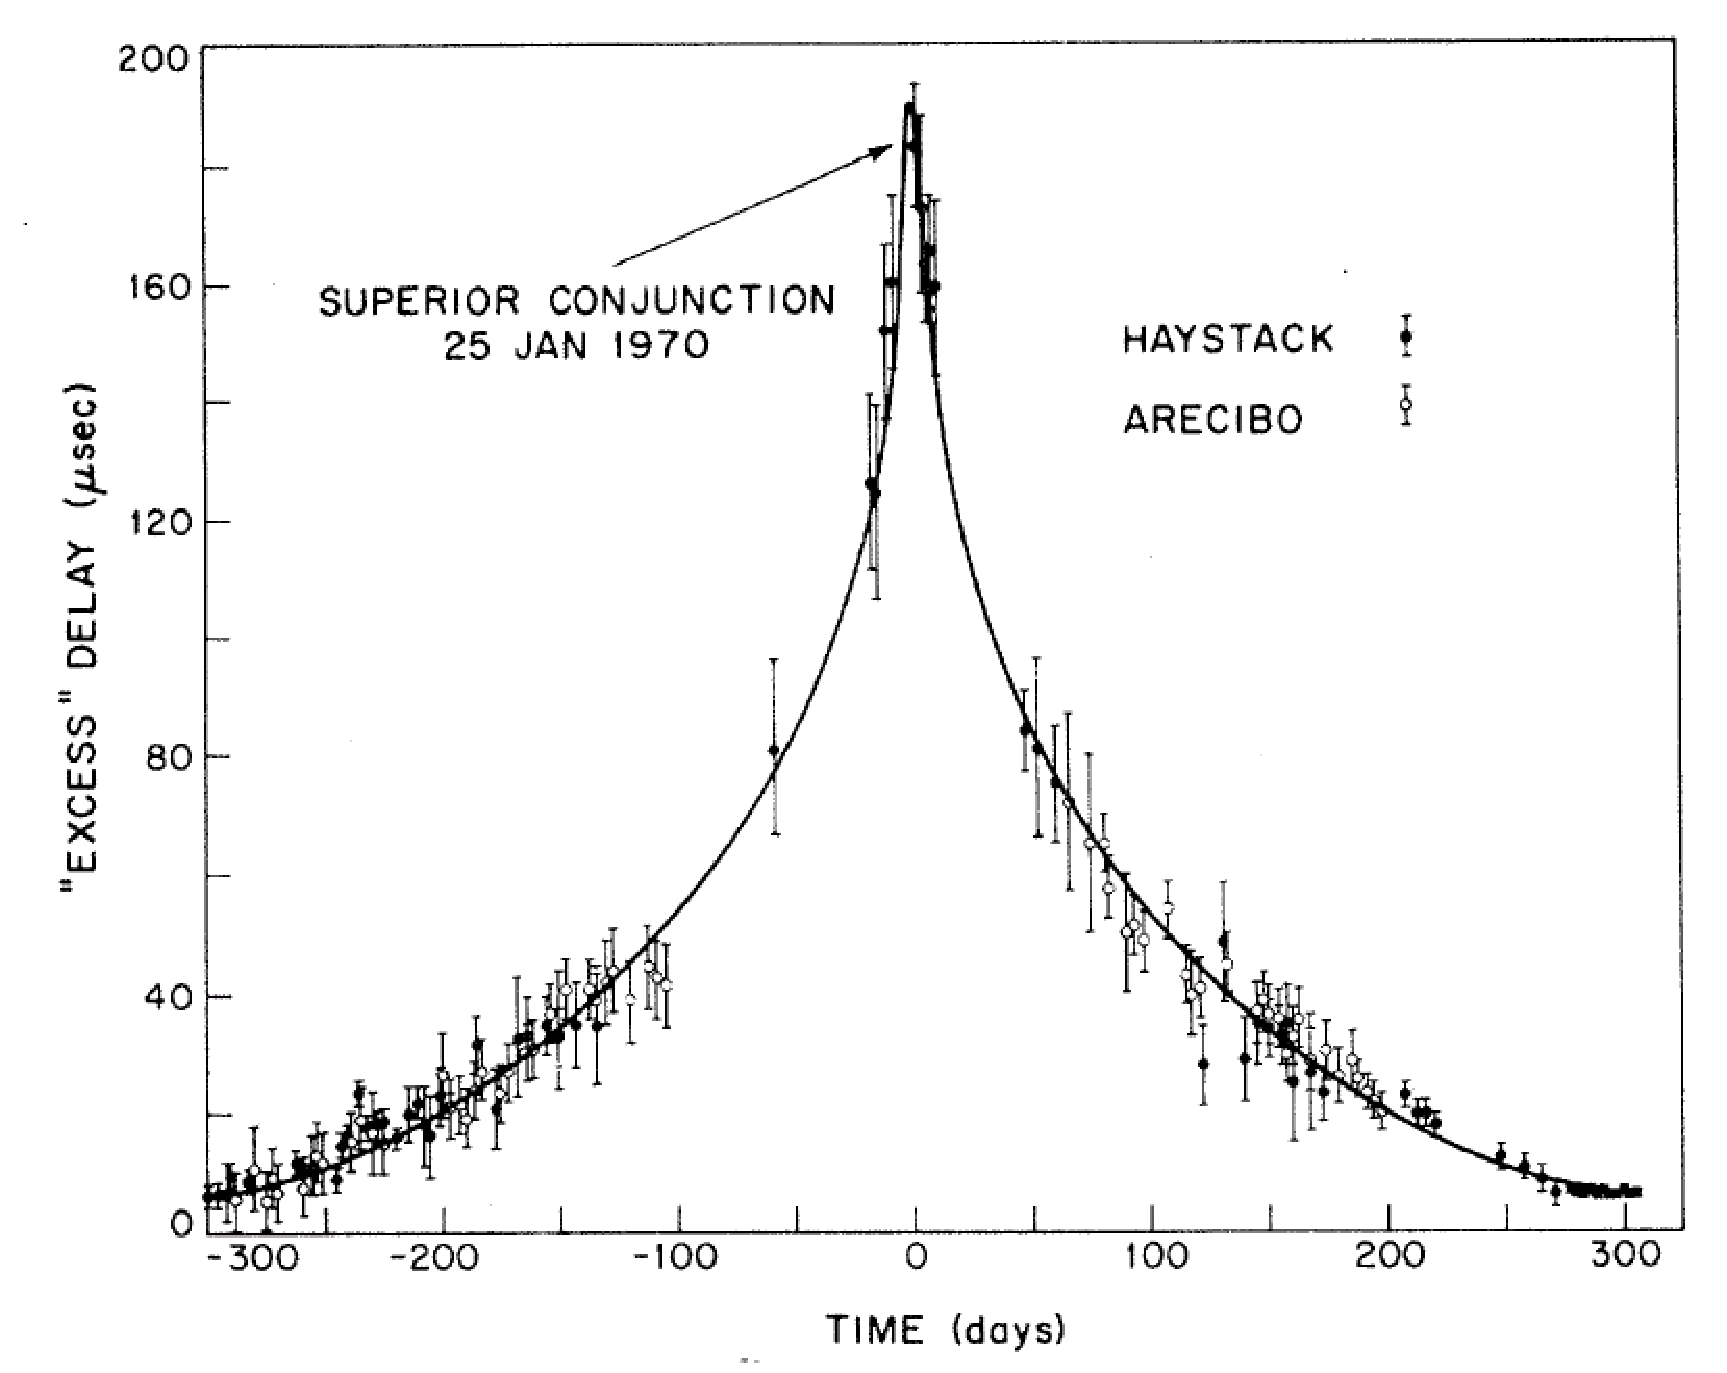
\includegraphics[height=6cm]{fig/fig-shapiro-delay-2.pdf}
\caption{Mediciones de Radar del efecto Shapiro.}
\end{center}
\end{figure}
